% !TeX program = xelatex
% Compile with XeLaTeX (fontspec + Korean text).
% Shared Beamer style and diagrams. Compile language files with XeLaTeX.
\documentclass[aspectratio=169,10pt]{beamer}
\usepackage[no-math]{fontspec}
\setsansfont{Malgun Gothic}
\setmainfont{Malgun Gothic}
\setmonofont{Consolas}
\XeTeXlinebreaklocale "ko"
\XeTeXlinebreakskip=0pt plus 0.5pt
\usepackage{amsmath,graphicx,booktabs,tikz}
\usefonttheme{professionalfonts}
\usefonttheme[onlymath]{serif}
\usetikzlibrary{arrows.meta,positioning,calc,shapes.geometric}
\definecolor{ink}{HTML}{142938}
\definecolor{accent}{HTML}{155F85}
\definecolor{pale}{HTML}{E7F0F7}
\definecolor{collision}{HTML}{A03336}
\setbeamercolor{normal text}{fg=ink,bg=white}
\setbeamercolor{frametitle}{fg=ink}
\setbeamercolor{structure}{fg=accent}
\setbeamerfont{frametitle}{size=\Large,series=\bfseries}
\setbeamertemplate{navigation symbols}{}
\setbeamertemplate{footline}{\hfill{\color{accent}\scriptsize RMFS Architecture\quad \insertframenumber\ /\ \inserttotalframenumber}\hspace{5mm}\vspace{3mm}}
\setbeamersize{text margin left=7mm,text margin right=7mm}
\hypersetup{pdftitle={RMFS Architecture}}
\tikzset{
 phase/.style={ellipse,draw=accent,fill=pale,minimum width=23mm,minimum height=10mm,align=center,font=\small},
 terminal/.style={phase,draw=collision,fill=red!5},
 flow/.style={-{Stealth[length=2mm]},draw=accent,thick},
 ext/.style={flow,dashed},
 crash/.style={ext,draw=collision},
 lab/.style={font=\scriptsize,align=center,fill=white,inner sep=1.5pt},
 module/.style={draw=accent,fill=pale,rounded corners=2pt,minimum width=34mm,minimum height=13mm,align=center}
}
\newcommand{\MRobotDiagram}{%
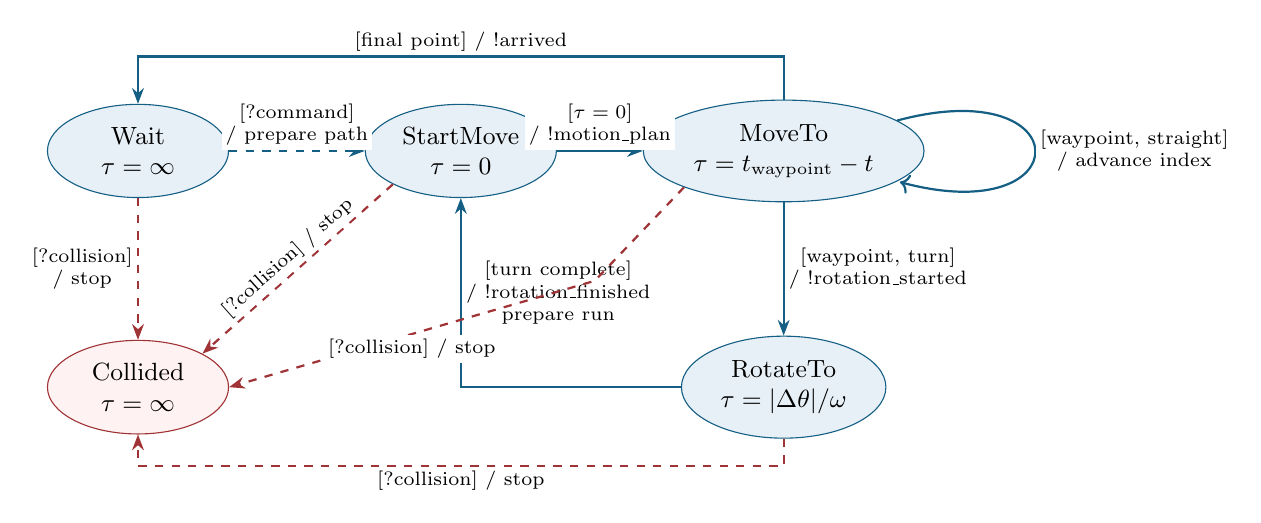
\begin{tikzpicture}[x=1cm,y=1cm]
\node[phase] (w) at (0,3) {Wait\\$\tau=\infty$};
\node[phase] (s) at (4.1,3) {StartMove\\$\tau=0$};
\node[phase] (m) at (8.2,3) {MoveTo\\$\tau=t_{\rm waypoint}-t$};
\node[phase] (r) at (8.2,0) {RotateTo\\$\tau=|\Delta\theta|/\omega$};
\node[terminal] (c) at (0,0) {Collided\\$\tau=\infty$};
\draw[ext] (w)--node[lab,above]{[?command]\\ / prepare path}(s);
\draw[flow] (s)--node[lab,above]{[$\tau=0$]\\ / !motion\_plan}(m);
\draw[flow] (m) edge[loop right] node[lab,right]{[waypoint, straight]\\ / advance index}(m);
\draw[flow] (m)--node[lab,right]{[waypoint, turn]\\ / !rotation\_started}(r);
\draw[flow] (r.west)--(4.1,0) -- node[lab,right]{[turn complete]\\ / !rotation\_finished\\prepare run}(s.south);
\draw[flow] (m.north)--(8.2,4.2)--node[lab,above]{[final point] / !arrived}(0,4.2)--(w.north);
\draw[crash] (w.south)--node[lab,left]{[?collision]\\ / stop}(c.north);
\draw[crash] (s.south west)--node[lab,above,sloped]{[?collision] / stop}(c.north east);
\draw[crash] (m.south west)--(5.8,1.35)--node[lab,below]{[?collision] / stop}(c.east);
\draw[crash] (r.south)--(8.2,-1)--node[lab,below]{[?collision] / stop}(0,-1)--(c.south);
\end{tikzpicture}}
\newcommand{\PSensorDiagram}{%
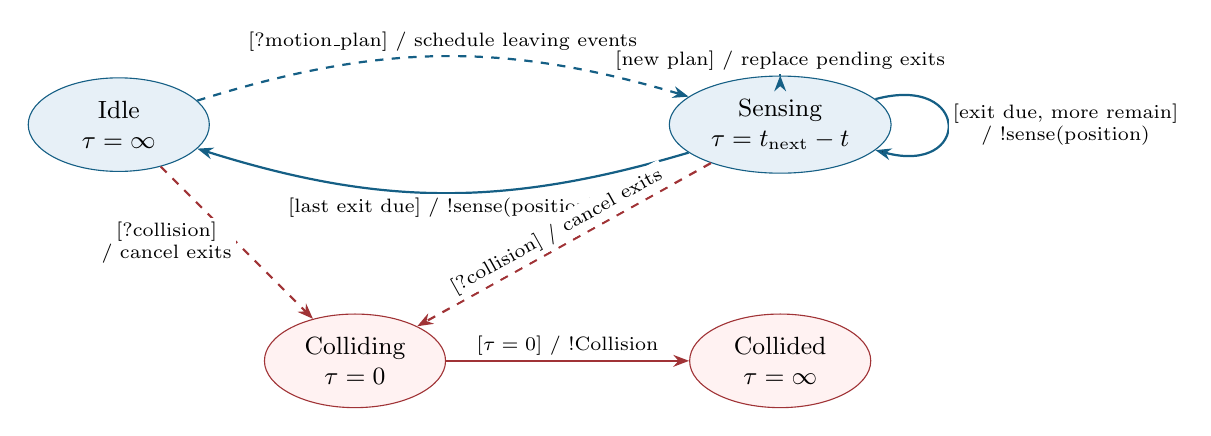
\begin{tikzpicture}[x=1cm,y=1cm]
\node[phase] (i) at (0,3) {Idle\\$\tau=\infty$};
\node[phase] (s) at (8.4,3) {Sensing\\$\tau=t_{\rm next}-t$};
\node[terminal] (g) at (3,0) {Colliding\\$\tau=0$};
\node[terminal] (c) at (8.4,0) {Collided\\$\tau=\infty$};
\draw[ext] (i) to[bend left=17] node[lab,above]{[?motion\_plan] / schedule leaving events}(s);
\draw[flow] (s) to[bend left=17] node[lab,below]{[last exit due] / !sense(position)}(i);
\draw[flow] (s) edge[loop right,looseness=5] node[lab,right]{[exit due, more remain]\\ / !sense(position)}(s);
\draw[ext] (s.north) to[out=120,in=60,looseness=3] node[lab,above]{[new plan] / replace pending exits}(s.north);
\draw[crash] (i)--node[lab,left]{[?collision]\\ / cancel exits}(g);
\draw[crash] (s)--node[lab,sloped,above]{[?collision] / cancel exits}(g);
\draw[flow,draw=collision] (g)--node[lab,above]{[$\tau=0$] / !Collision}(c);
\end{tikzpicture}}
\newcommand{\Profiles}{%
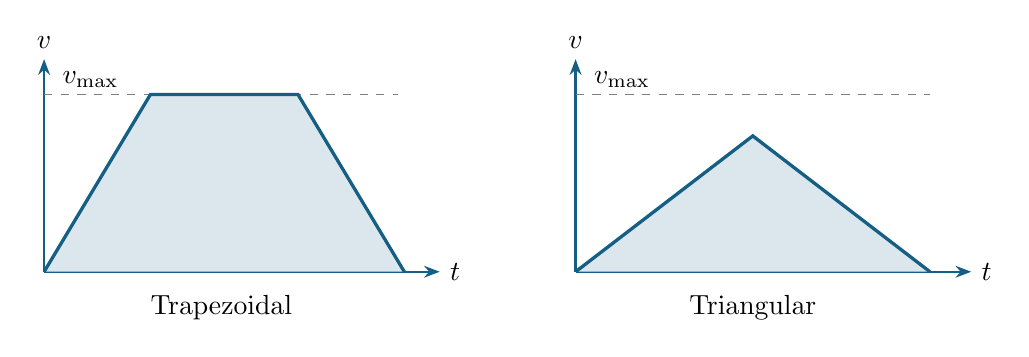
\begin{tikzpicture}[x=0.75cm,y=0.75cm]
\foreach \x in {0,9}{
 \draw[flow] (\x,0)--++(6.7,0) node[right] {$t$};
 \draw[flow] (\x,0)--++(0,3.6) node[above] {$v$};
 \draw[dashed,gray] (\x,3)--++(6,0);
}
\fill[accent!15] (0,0)--(1.8,3)--(4.3,3)--(6.1,0)--cycle;
\draw[accent,very thick] (0,0)--(1.8,3)--(4.3,3)--(6.1,0);
\fill[accent!15] (9,0)--(12,2.3)--(15,0)--cycle;
\draw[accent,very thick] (9,0)--(12,2.3)--(15,0);
\node at (3,-.6) {Trapezoidal};
\node at (12,-.6) {Triangular};
\node[anchor=west] at (.15,3.25) {$v_{\max}$};
\node[anchor=west] at (9.15,3.25) {$v_{\max}$};
\end{tikzpicture}}
\newcommand{\shot}[1]{\includegraphics[width=\linewidth,height=5.65cm,keepaspectratio]{assets/#1.png}}


\usetikzlibrary{decorations.pathreplacing}
\title{RMFS Architecture}
\date{2026-11-18}
\begin{document}

\begin{frame}[plain]
\centering
{\color{accent}\LARGE Part 1\par}\vspace{8mm}
{\LARGE Introduction to RMFS\par Modeling and Control\par}
\end{frame}


\begin{frame}{RMFS Architecture}

\begin{center}
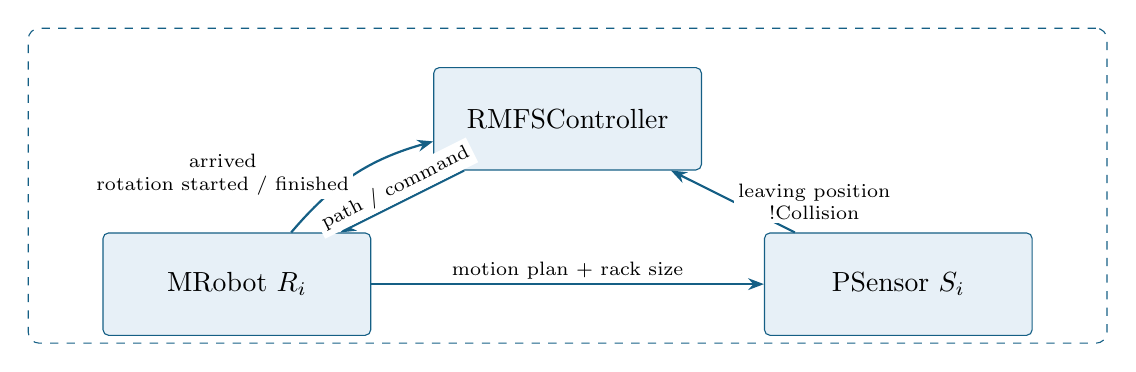
\begin{tikzpicture}
\node[module] (c) at (0,2.1) {RMFSController};
\node[module] (r) at (-4.2,0) {MRobot $R_i$};
\node[module] (s) at (4.2,0) {PSensor $S_i$};
\draw[flow] (c)--node[lab,above,sloped]{path / command}(r);
\draw[flow] (r) to[bend left=17] node[lab,left]{arrived\\rotation started / finished}(c);
\draw[flow] (r)--node[lab,above]{motion plan + rack size}(s);
\draw[flow] (s)--node[lab,right]{leaving position\\!Collision}(c);
\node[draw=accent,dashed,rounded corners,minimum width=13.7cm,minimum height=4cm] at (0,1.25) {};
\end{tikzpicture}
\end{center}

\small RMFS is a Coupled DEVS containing a controller and one MRobot--PSensor pair per physical robot.
MRobot executes motion. PSensor reports clearance positions. The 3D rendering of MRobot is affectionately called \textbf{Frogeye (Frogy)}.
The current experiments use \texttt{TestController}; the planned RMFSController contains
RobotPathPlanner, TrafficManager and their shared RoadMap.\par\smallskip Grid: $4\times4$ control points, $3\times3$ cells, 2 m spacing, $6\times6$ m.
\end{frame}

\begin{frame}{MRobot phase transitions}
\centering\resizebox{.95\linewidth}{!}{\MRobotDiagram}
\par\medskip\raggedright\small
Edges use [guard] / action. Dashed edges process external input.
Each straight run accelerates and brakes once. Intermediate collinear waypoints preserve speed.
On collision, freeze pose and cancel motion. The rack keeps its orientation during body rotation.
{\scriptsize $t$ is current time, $t_{\rm waypoint}$ the next waypoint time, $\Delta\theta$ the turn angle and $\omega$ the turn rate.}
\end{frame}

\begin{frame}{PSensor phase transitions}
\centering\resizebox{!}{4.2cm}{\PSensorDiagram}
\par\medskip\raggedright\small
Only leaving events are scheduled. \texttt{!sense} carries the robot-center coordinates at clearance.
A new motion plan replaces pending exits.
A collision cancels exits, then reports \texttt{!Collision} at the same simulation time.
If no exit is scheduled, the next-event time is infinite. $t_{\rm next}$ is the next exit time and $t$ current time.
\end{frame}

\begin{frame}{MRobot velocity profiles}
\begin{center}\resizebox{.82\linewidth}{!}{\Profiles}\end{center}
\[
v_p=\min\!\left(v_{\max},\sqrt{\frac{2D}{1/a+1/b}}\right),
\qquad d_a=\frac{v_p^2}{2a},\quad d_b=\frac{v_p^2}{2b}.
\]
\[
T=\frac{v_p}{a}+\frac{D-d_a-d_b}{v_p}+\frac{v_p}{b},
\qquad T_{\rm turn}=\frac{|\Delta\theta|}{\omega}.
\]
\footnotesize
$D$ is the total distance of one uninterrupted straight run [m].
$a,b>0$ are acceleration and braking magnitudes [m/s$^2$].
$v_{\max}$ is the speed limit and $v_p$ the attained peak speed [m/s].
$d_a,d_b$ are acceleration and braking distances [m].
$T$ is the run duration [s]. $\Delta\theta$ is the heading change
and $\omega$ the turn rate, expressed in matching angular units.
\end{frame}

\begin{frame}{PSensor clearance on a commanded path}

\begin{center}
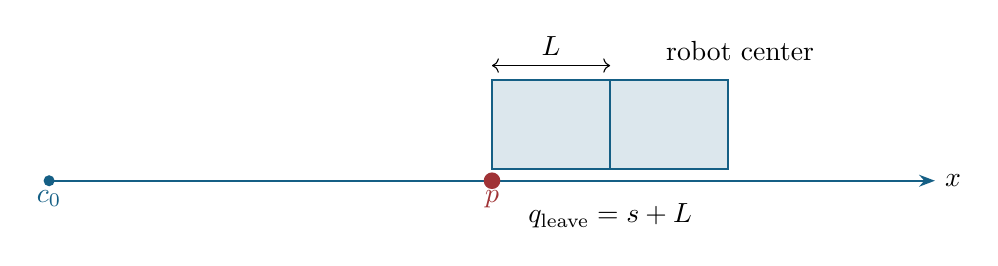
\begin{tikzpicture}[x=.75cm,y=.75cm]
\draw[flow] (0,0)--(15,0) node[right] {$x$};
\fill[accent!15] (7.5,.2) rectangle (11.5,1.7);
\draw[accent,thick] (7.5,.2) rectangle (11.5,1.7);
\draw[accent,thick] (9.5,.2)--(9.5,1.7);
\node at (11.7,2.2) {robot center};
\draw[<->] (7.5,1.95)--node[above] {$L$}(9.5,1.95);
\fill[collision] (7.5,0) circle (3pt) node[below] {$p$};
\fill[accent] (0,0) circle (2pt) node[below] {$c_0$};
\node at (9.5,-.6) {$q_{\rm leave}=s+L$};
\end{tikzpicture}
\end{center}

\[
s=(p-c_0)\cdot u,\qquad q_{\rm leave}=s+L,\qquad
t_{\rm leave}=t_0+T(q_{\rm leave}).
\]
\footnotesize
$p$ is the control-point coordinate, $c_0$ the center at run start $t_0$,
and $u$ the unit motion direction. $s$ is the signed distance to $p$ along the run.
$q_{\rm leave}$ is center travel from $c_0$ to clearance.
$T(q)$ is elapsed travel time and $t_{\rm leave}$ the absolute event time.
The message carries $c_{\rm leave}=c_0+u q_{\rm leave}$ in metres.
\par\medskip
\textbf{$L=0.75$ m for both loaded and empty robots in these tests.}
It comes from the constructor's 1.5 m rack dimension.
Schedule when $0\le q_{\rm leave}<D$.
A stop-point exit is reconsidered on the next run.

\end{frame}

\begin{frame}{Clearance time under acceleration, cruise and braking}
\[
T(q)=
\begin{cases}
\sqrt{\dfrac{2q}{a}},&0\le q\le d_a,\\[2mm]
\dfrac{v_p}{a}+\dfrac{q-d_a}{v_p},&d_a<q<D-d_b,\\[2mm]
T-\sqrt{\dfrac{2(D-q)}{b}},&D-d_b\le q\le D .
\end{cases}
\]
\footnotesize $q$ is center travel from run start; $T(q)$ is its elapsed arrival time.
$D,a,b,v_p,d_a,d_b,T$ are defined on page 4.
Set $q=s+L$; a departure point has $s=0$.
\[
\text{Example}\quad L=0.75\ {\rm m},\ a=b=0.41\ {\rm m/s^2}
\ \Rightarrow\ T(L)=1.912730\ {\rm s}.
\]
\small Compute event times analytically when the run starts. The engine advances to those events.
The Viewer samples positions for animation.
\end{frame}

\begin{frame}{RMFSController composition}
\begin{center}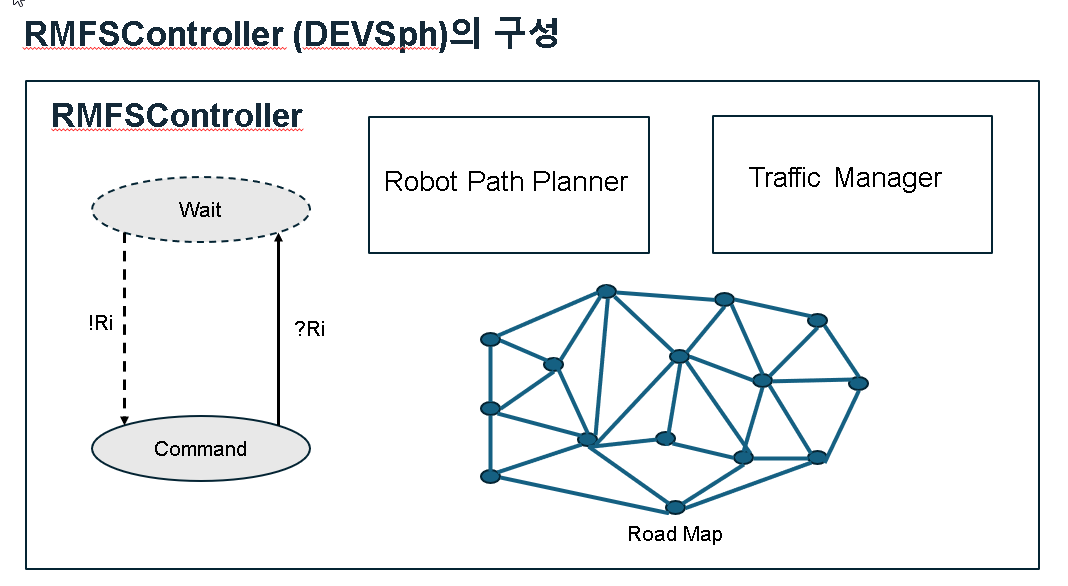
\includegraphics[width=.88\linewidth,height=5.4cm,keepaspectratio]{assets/RMFSController.png}\end{center}
\small Author-supplied design figure. RobotPathPlanner and TrafficManager share RoadMap.
Current tests use TestController. Controller phase transitions are deferred.
\end{frame}

\begin{frame}{Frogy -- Straight}
\begin{columns}[T,onlytextwidth]
\begin{column}{.70\textwidth}\shot{straight}\end{column}
\begin{column}{.28\textwidth}\small Path $(0,2)\to(3,2)$\par\medskip Distance 6 m\par Turns 0\par Rack OFF\par\medskip\textbf{Running time}\par\textbf{7.651 s}\par\medskip Snapshot $t=3.800$ s.\end{column}
\end{columns}
\vspace{1mm}
{\tiny\texttt{\detokenize{01_01_RobotPath_Straight}}\par \texttt{\detokenize{python -m examples.RMFS.Tests.01_01_RobotPath_Straight --no-rack}}\par Empty robot. Initial heading follows the first segment. $v_{\max}=2\,\mathrm{m/s}$, $a=b=0.41\,\mathrm{m/s^2}$, $\omega=45^\circ/\mathrm{s}$.}
\end{frame}

\begin{frame}{Frogy -- ZigZag}
\begin{columns}[T,onlytextwidth]
\begin{column}{.70\textwidth}\shot{zigzag}\end{column}
\begin{column}{.28\textwidth}\small Path $(0,3)\to(1,3)\to(1,2)\to\cdots\to(3,0)$\par\medskip Distance 12 m\par Turns 5\par Rack OFF\par\medskip\textbf{Running time}\par\textbf{36.504 s}\par\medskip Snapshot $t=18.000$ s.\end{column}
\end{columns}
\vspace{1mm}
{\tiny\texttt{\detokenize{01_02_RobotPath_LeftTop_RightBottom_ZigZag}}\par \texttt{\detokenize{python -m examples.RMFS.Tests.01_02_RobotPath_LeftTop_RightBottom_ZigZag --no-rack}}\par Empty robot. Initial heading follows the first segment. $v_{\max}=2\,\mathrm{m/s}$, $a=b=0.41\,\mathrm{m/s^2}$, $\omega=45^\circ/\mathrm{s}$.}
\end{frame}

\begin{frame}{Frogy -- L-shaped path}
\begin{columns}[T,onlytextwidth]
\begin{column}{.70\textwidth}\shot{lpath}\end{column}
\begin{column}{.28\textwidth}\small Path $(0,3)\to(0,0)\to(3,0)$\par\medskip Distance 12 m\par Turns 1\par Rack OFF\par\medskip\textbf{Running time}\par\textbf{17.302 s}\par\medskip Snapshot $t=8.500$ s.\end{column}
\end{columns}
\vspace{1mm}
{\tiny\texttt{\detokenize{01_03_RobotPath_LeftTop_RightBottom_Straight_L}}\par \texttt{\detokenize{python -m examples.RMFS.Tests.01_03_RobotPath_LeftTop_RightBottom_Straight_L --no-rack}}\par Empty robot. Initial heading follows the first segment. $v_{\max}=2\,\mathrm{m/s}$, $a=b=0.41\,\mathrm{m/s^2}$, $\omega=45^\circ/\mathrm{s}$.}
\end{frame}

\begin{frame}{Frogy -- Round trip}
\begin{columns}[T,onlytextwidth]
\begin{column}{.70\textwidth}\shot{roundtrip}\end{column}
\begin{column}{.28\textwidth}\small Path $(0,2)\to(2,2)\to(0,2)$\par\medskip Distance 8 m\par Turns 1\par Rack OFF\par\medskip\textbf{Running time}\par\textbf{16.494 s}\par\medskip Snapshot $t=8.200$ s.\end{column}
\end{columns}
\vspace{1mm}
{\tiny\texttt{\detokenize{01_04_RobotPath_RoundTrip}}\par \texttt{\detokenize{python -m examples.RMFS.Tests.01_04_RobotPath_RoundTrip --no-rack}}\par Empty robot. Initial heading follows the first segment. $v_{\max}=2\,\mathrm{m/s}$, $a=b=0.41\,\mathrm{m/s^2}$, $\omega=45^\circ/\mathrm{s}$.}
\end{frame}



\begin{frame}{Frogy -- L path and retraced L return}
\begin{columns}[T,onlytextwidth]
\begin{column}{.70\textwidth}\shot{backward_l}\end{column}
\begin{column}{.28\textwidth}\small Path $(0,3)\to(0,0)\to(3,0)\to(0,0)\to(0,3)$\par\medskip Distance 24 m\par Rack OFF\par Turns $90^\circ,180^\circ,90^\circ$\par\medskip\textbf{Running time}\par\textbf{38.604 s}\par\medskip Snapshot $t=19.300$ s.\end{column}
\end{columns}
\vspace{1mm}
{\tiny\texttt{\detokenize{01_05_RobotPath_L_backward_L}}\par
\texttt{\detokenize{python -m examples.RMFS.Tests.01_05_RobotPath_L_backward_L}}\par
4 straight runs of 6 m; initial heading south. Final heading north. $\omega=45^\circ/\mathrm{s}$. $T=4\mathcal T(6;0,0)+360^\circ/\omega=38.603682\,\mathrm{s}$.}
\end{frame}

\begin{frame}{Frogy -- L path and perimeter return}
\begin{columns}[T,onlytextwidth]
\begin{column}{.70\textwidth}\shot{rotate_l}\end{column}
\begin{column}{.28\textwidth}\small Path $(0,3)\to(0,0)\to(3,0)\to(3,3)\to(0,3)$\par\medskip Distance 24 m\par Rack OFF\par Turns $90^\circ,90^\circ,90^\circ$\par\medskip\textbf{Running time}\par\textbf{36.604 s}\par\medskip Snapshot $t=18.300$ s.\end{column}
\end{columns}
\vspace{1mm}
{\tiny\texttt{\detokenize{01_06_RobotPath_L_rotate_L}}\par
\texttt{\detokenize{python -m examples.RMFS.Tests.01_06_RobotPath_L_rotate_L}}\par
4 straight runs of 6 m; initial heading south. Final heading west. $\omega=45^\circ/\mathrm{s}$. $T=4\mathcal T(6;0,0)+270^\circ/\omega=36.603682\,\mathrm{s}$. The 2 s saving is entirely rotation time.}
\end{frame}

\begin{frame}
\frametitle{\large Future Work: Building Motion Time edge Graph}
\begin{columns}[T,onlytextwidth]
\begin{column}{.36\textwidth}
\begin{center}

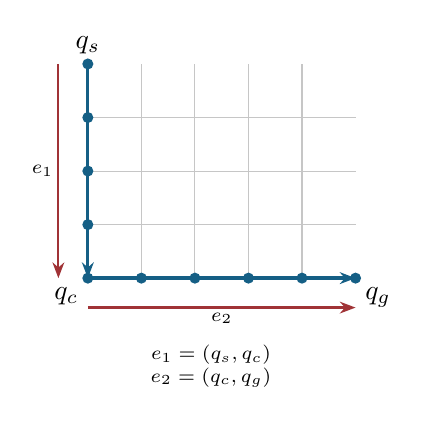
\begin{tikzpicture}[x=.68cm,y=.68cm]
\foreach \y in {1,2,3}{\draw[gray!45] (0,\y)--(5,\y);}
\foreach \x in {1,2,3,4}{\draw[gray!45] (\x,0)--(\x,4);}
\draw[flow,very thick] (0,4)--(0,0);
\draw[flow,very thick] (0,0)--(5,0);
\foreach \y in {0,1,2,3,4}{\fill[accent] (0,\y) circle (2pt);}
\foreach \x in {1,2,3,4,5}{\fill[accent] (\x,0) circle (2pt);}
\node[above] at (0,4) {$q_s$};
\node[below left] at (0,0) {$q_c$};
\node[below right] at (5,0) {$q_g$};
\draw[flow,draw=collision,thick] (-.55,4)--node[lab,left] {$e_1$}(-.55,0);
\draw[flow,draw=collision,thick] (0,-.55)--node[lab,below] {$e_2$}(5,-.55);
\node[align=center,font=\scriptsize] at (2.3,-1.65) {$e_1=(q_s,q_c)$\\$e_2=(q_c,q_g)$};
\end{tikzpicture}

\end{center}
\end{column}
\begin{column}{.62\textwidth}
\footnotesize Add two straight direct edges $e_1$ and $e_2$. Every edge, including original grid edges, gets a motion-profile travel time.
\[
w(e)=\mathcal T_{\rm motion}
       (d_e;\,v_e^{\rm in},v_e^{\rm out},a,b,v_{\max})
\]
\[
w(e_1)=\mathcal T(d_1;0,0),\qquad
w(e_2)=\mathcal T(d_2;0,0)
\]
\[
C_{\rm turn}(e_i,e_{i+1})=
\frac{|\Delta\theta(e_i,e_{i+1})|}{\omega},
\quad |\Delta\theta|\in\{0^\circ,90^\circ,180^\circ\}.
\]
\[
\boxed{C(P)=\sum_{e\in P}w(e)+
\sum_{(e_i,e_{i+1})\in P}C_{\rm turn}(e_i,e_{i+1})}
\]
\[
d_1=d_2=6\,{\rm m}:\quad
7.651+\frac{90^\circ}{45^\circ/{\rm s}}+7.651
=17.302\,{\rm s}.
\]
\end{column}
\end{columns}
\medskip
\footnotesize $d_e$ is edge length; $v_e^{\rm in},v_e^{\rm out}$ are endpoint speeds. $\theta_e$ is edge heading; $\Delta\theta$ is the smallest heading change. Collinear edges carry speed across the junction. A turn requires a stop. The planning state is $(p,\theta,v)$; each direct edge retains its intermediate control points. $P$ is the candidate path; $d_1,d_2$ are direct-edge lengths. $\mathcal T_{\rm motion}$ is profile travel time [s]; $\mathcal T(d;0,0)$ is the stop-to-stop duration on page 4.
\end{frame}

\begin{frame}{Counting direct edges through control points}
\begin{columns}[T,onlytextwidth]
\begin{column}{.40\textwidth}
\begin{center}

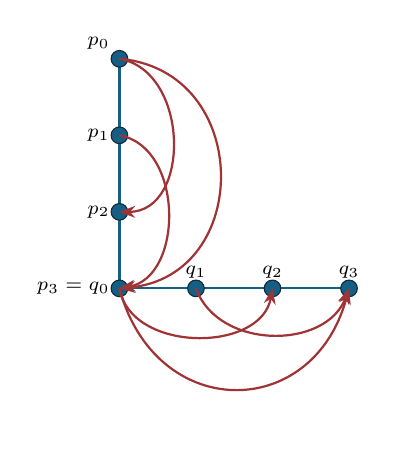
\begin{tikzpicture}[x=.54cm,y=.54cm]
\draw[accent,thick] (0,5.4)--(0,0)--(5.4,0);
\foreach \y in {0,1.8,3.6,5.4}{\filldraw[fill=accent,draw=ink] (0,\y) circle(3pt);}
\foreach \x in {1.8,3.6,5.4}{\filldraw[fill=accent,draw=ink] (\x,0) circle(3pt);}
\draw[flow,draw=collision] (0,5.4) to[out=-10,in=0,looseness=1.2] (0,1.8);
\draw[flow,draw=collision] (0,5.4) to[out=-5,in=5,looseness=1.5] (0,0);
\draw[flow,draw=collision] (0,3.6) to[out=-10,in=10,looseness=1.1] (0,0);
\draw[flow,draw=collision] (0,0) to[out=-80,in=-100,looseness=1.1] (3.6,0);
\draw[flow,draw=collision] (0,0) to[out=-75,in=-105,looseness=1.55] (5.4,0);
\draw[flow,draw=collision] (1.8,0) to[out=-70,in=-110,looseness=1.1] (5.4,0);
\node[above left,font=\scriptsize] at (0,5.4) {$p_0$};
\node[left,font=\scriptsize] at (0,3.6) {$p_1$};
\node[left,font=\scriptsize] at (0,1.8) {$p_2$};
\node[left,font=\scriptsize] at (0,0) {$p_3=q_0$};
\node[above,font=\scriptsize] at (1.8,0) {$q_1$};
\node[above,font=\scriptsize] at (3.6,0) {$q_2$};
\node[above,font=\scriptsize] at (5.4,0) {$q_3$};
\end{tikzpicture}

\end{center}
\end{column}
\begin{column}{.58\textwidth}
\small A straight line contains $n$ control points, including both ends. For one travel direction there are $\binom n2$ point pairs, of which $n-1$ already form adjacent grid edges.
\[
\boxed{E_{\rm add}^{\rightarrow}(n)
=\binom n2-(n-1)=\frac{(n-1)(n-2)}2}
\]
\[
E_{\rm add}^{\leftrightarrow}(n)=(n-1)(n-2).
\]

\begin{center}\small
\begin{tabular}{rrr}\toprule
Points $n$ & One direction & Both directions\\\midrule
4 & 3 & 6\\
10 & 36 & 72\\
20 & 171 & 342\\\bottomrule
\end{tabular}\end{center}

\end{column}
\end{columns}
\medskip
\footnotesize Blue segments are existing adjacent edges. Red arcs represent straight travel across at least one intermediate point. The figure has 3 red edges on each line, 6 total in the shown directions; adding reverse arcs gives 12.\par\smallskip The current $4\times4$ point grid has 8 straight rows/columns, adding $8\times6=48$ directed edges to 48 original arcs, for 96 total.
\end{frame}

\begin{frame}[plain]
\centering
{\color{accent}\LARGE Part 2\par}\vspace{8mm}
{\LARGE Traffic Management\par}
\end{frame}

\begin{frame}{Definition 1: paths and subpaths}
\small We \textbf{abstract away time while preserving path order and stage precedence}. Numerical times and speeds are introduced later for physical execution and performance evaluation.
\medskip\par
\normalsize A moving object's path is a continuous path from its initial to its final configuration.
\begin{equation}
P_i:[0,1]\longrightarrow\mathcal Q_i,\qquad p_i^s=P_i(0),\quad p_i^e=P_i(1).
\tag{1}
\end{equation}
\small $\mathcal Q_i$ is a configuration space, including position and orientation. The parameter $u\in[0,1]$ measures \textbf{path progress, not time}.
\medskip\par
\normalsize For $0\le a\le b\le1$, the subpath follows $P_i$ from $P_i(a)$ to $P_i(b)$ in its original order.
\begin{equation}
P_i^{[a,b]}:=P_i\big|_{[a,b]}.
\tag{2}
\end{equation}
\small Progress values distinguish separate visits even when the spatial position is the same.
\end{frame}

\begin{frame}{Definition 2: occupancy and subpath sweeps}
Let $B_i(u)$ be the region occupied by object $i$ at configuration $P_i(u)$.
\begin{equation}B_i(u)\subseteq\mathbb R^d,\qquad u\in[0,1].\tag{3}\end{equation}
The sweep of a subpath is the union of its occupied regions.
\begin{equation}S_i(P_i^{[a,b]}):=\bigcup_{u\in[a,b]}B_i(u).\tag{4}\end{equation}
\begin{center}
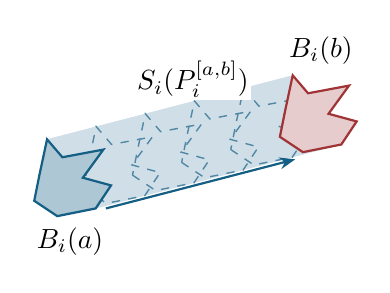
\begin{tikzpicture}[scale=.65]
\path[fill=accent!20,draw=none] (-0.8000,-0.3500)--(-0.3500,-0.6500)--(0.4000,-0.5000)--(0.7000,-0.0500)--(0.1500,0.1000)--(0.5500,0.6500)--(-0.2500,0.5000)--(-0.5500,0.8500)--(-0.7000,0.1500)--cycle;
\path[fill=accent!20,draw=none] (4.0000,0.9000)--(4.4500,0.6000)--(5.2000,0.7500)--(5.5000,1.2000)--(4.9500,1.3500)--(5.3500,1.9000)--(4.5500,1.7500)--(4.2500,2.1000)--(4.1000,1.4000)--cycle;
\path[fill=accent!20,draw=none] (-0.8000,-0.3500)--(-0.3500,-0.6500)--(4.4500,0.6000)--(4.0000,0.9000)--cycle;
\path[fill=accent!20,draw=none] (-0.3500,-0.6500)--(0.4000,-0.5000)--(5.2000,0.7500)--(4.4500,0.6000)--cycle;
\path[fill=accent!20,draw=none] (0.4000,-0.5000)--(0.7000,-0.0500)--(5.5000,1.2000)--(5.2000,0.7500)--cycle;
\path[fill=accent!20,draw=none] (0.7000,-0.0500)--(0.1500,0.1000)--(4.9500,1.3500)--(5.5000,1.2000)--cycle;
\path[fill=accent!20,draw=none] (0.1500,0.1000)--(0.5500,0.6500)--(5.3500,1.9000)--(4.9500,1.3500)--cycle;
\path[fill=accent!20,draw=none] (0.5500,0.6500)--(-0.2500,0.5000)--(4.5500,1.7500)--(5.3500,1.9000)--cycle;
\path[fill=accent!20,draw=none] (-0.2500,0.5000)--(-0.5500,0.8500)--(4.2500,2.1000)--(4.5500,1.7500)--cycle;
\path[fill=accent!20,draw=none] (-0.5500,0.8500)--(-0.7000,0.1500)--(4.1000,1.4000)--(4.2500,2.1000)--cycle;
\path[fill=accent!20,draw=none] (-0.7000,0.1500)--(-0.8000,-0.3500)--(4.0000,0.9000)--(4.1000,1.4000)--cycle;
\begin{scope}[shift={(0.960,0.250)}]\draw[accent!75,dashed,line width=.5pt] (-0.8000,-0.3500)--(-0.3500,-0.6500)--(0.4000,-0.5000)--(0.7000,-0.0500)--(0.1500,0.1000)--(0.5500,0.6500)--(-0.2500,0.5000)--(-0.5500,0.8500)--(-0.7000,0.1500)--cycle;\end{scope}
\begin{scope}[shift={(1.920,0.500)}]\draw[accent!75,dashed,line width=.5pt] (-0.8000,-0.3500)--(-0.3500,-0.6500)--(0.4000,-0.5000)--(0.7000,-0.0500)--(0.1500,0.1000)--(0.5500,0.6500)--(-0.2500,0.5000)--(-0.5500,0.8500)--(-0.7000,0.1500)--cycle;\end{scope}
\begin{scope}[shift={(2.880,0.750)}]\draw[accent!75,dashed,line width=.5pt] (-0.8000,-0.3500)--(-0.3500,-0.6500)--(0.4000,-0.5000)--(0.7000,-0.0500)--(0.1500,0.1000)--(0.5500,0.6500)--(-0.2500,0.5000)--(-0.5500,0.8500)--(-0.7000,0.1500)--cycle;\end{scope}
\begin{scope}[shift={(3.840,1.000)}]\draw[accent!75,dashed,line width=.5pt] (-0.8000,-0.3500)--(-0.3500,-0.6500)--(0.4000,-0.5000)--(0.7000,-0.0500)--(0.1500,0.1000)--(0.5500,0.6500)--(-0.2500,0.5000)--(-0.5500,0.8500)--(-0.7000,0.1500)--cycle;\end{scope}
\path[fill=accent!35,draw=accent,thick] (-0.8000,-0.3500)--(-0.3500,-0.6500)--(0.4000,-0.5000)--(0.7000,-0.0500)--(0.1500,0.1000)--(0.5500,0.6500)--(-0.2500,0.5000)--(-0.5500,0.8500)--(-0.7000,0.1500)--cycle;
\begin{scope}[shift={(4.8,1.25)}]\path[fill=collision!25,draw=collision,thick] (-0.8000,-0.3500)--(-0.3500,-0.6500)--(0.4000,-0.5000)--(0.7000,-0.0500)--(0.1500,0.1000)--(0.5500,0.6500)--(-0.2500,0.5000)--(-0.5500,0.8500)--(-0.7000,0.1500)--cycle;\end{scope}
\draw[flow] (.6,-.5)--(4.3,.46);
\node[below] at (-.1,-.68) {$B_i(a)$};
\node[above] at (4.8,2.12) {$B_i(b)$};
\node[above,fill=white,inner sep=1pt] at (2.3,1.6) {$S_i(P_i^{[a,b]})$};
\end{tikzpicture}
\end{center}
\small An irregular polygon translates diagonally. The full sweep is the same operation with $a=0,b=1$. Here $d=2$ for the plane and $d=3$ for space. A conservative approximation must contain the actual sweep.
\end{frame}

\begin{frame}{Example: full and partial RMFS sweeps}
\small The rack remains axis-aligned when the robot body turns. For rack side length $2L_i$ and center $p_i(u)$,
\begin{equation}B_i(u)=p_i(u)+[-L_i,L_i]^2.\tag{5}\end{equation}
\small if $P_i^{[a,b]}$ is a horizontal or vertical straight segment,
\begin{equation}S_i(P_i^{[a,b]})=[p_i(a),p_i(b)]\oplus[-L_i,L_i]^2.\tag{6}\end{equation}
\begin{columns}[T]
\begin{column}{.49\textwidth}\centering
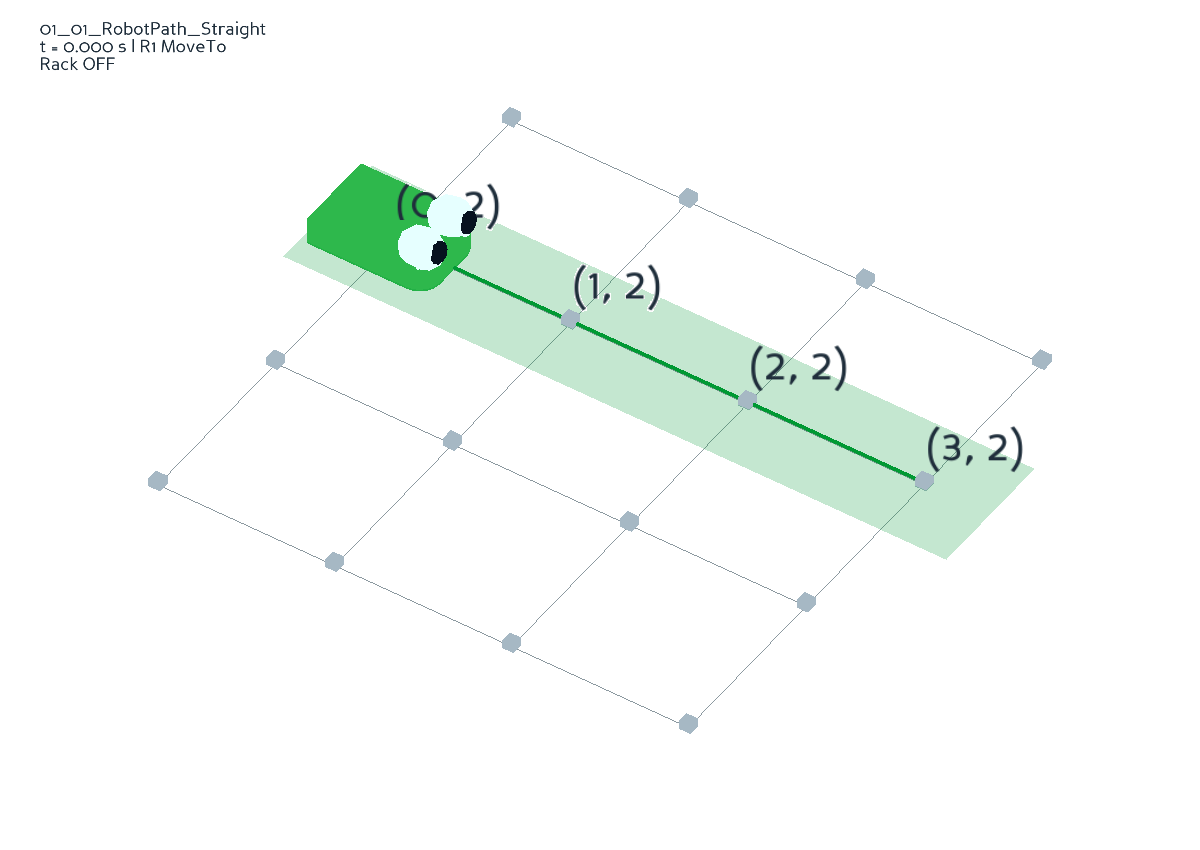
\includegraphics[height=2.65cm,keepaspectratio]{assets/straight_white_sweep.png}\par
{\scriptsize Full path: $(0,2)$ to $(3,2)$.}
\end{column}\begin{column}{.49\textwidth}\centering
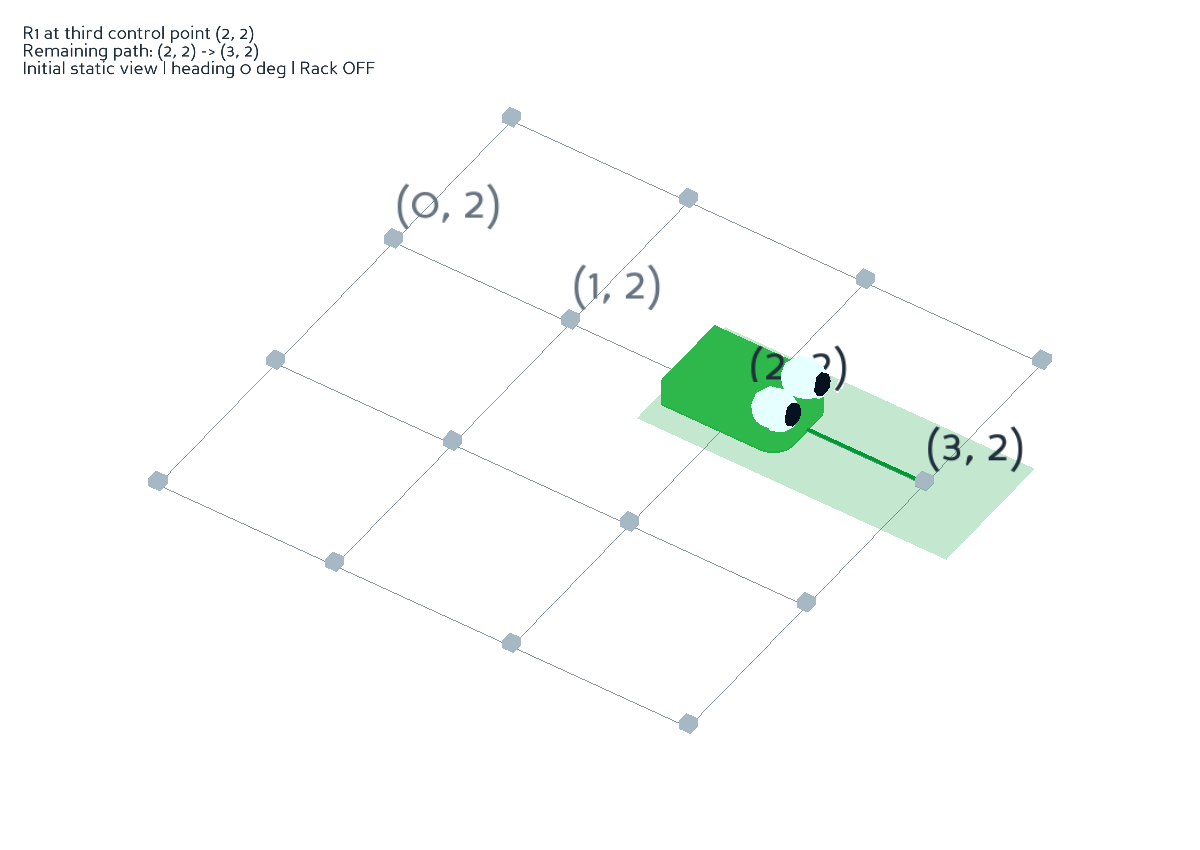
\includegraphics[height=2.65cm,keepaspectratio]{assets/remaining_straight_third_point.png}\par
{\scriptsize Subpath: $(2,2)$ to $(3,2)$.}
\end{column}\end{columns}
\small $\oplus$ denotes the Minkowski sum. A center displacement of $\ell$ produces a rectangle of length $\ell+2L_i$ and width $2L_i$, including both endpoint footprints. Coordinates are grid point indices.
\end{frame}

\begin{frame}{Definition 3: point paths and waiting}
Equal endpoint progress values define a \textbf{point path}: the configuration does not change. It represents waiting during that stage.
\begin{equation}
P_i^{[a,a]}:\ \text{wait at }P_i(a),\qquad S_i(P_i^{[a,a]})=B_i(a).
\tag{7}
\end{equation}
\begin{center}
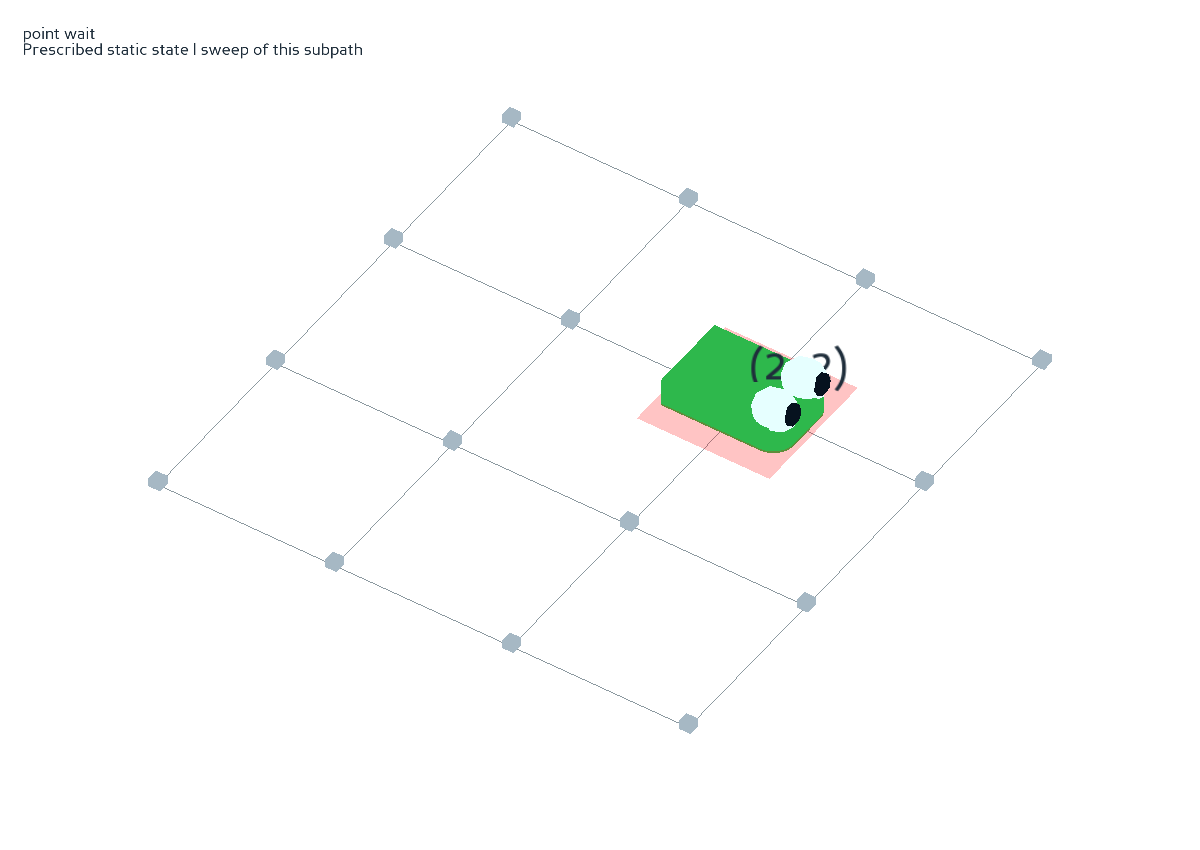
\includegraphics[height=3.0cm,keepaspectratio]{assets/point_wait_white.png}\par
{\scriptsize The point-path sweep of an object at grid point $(2,2)$.}
\end{center}
\small Waiting does not remove occupancy. The square footprint remains even without motion, so a waiting object participates in the same sweep-intersection test.
\end{frame}

\begin{frame}{Definition 4: ordered decomposition with waiting}
Divide each path into finitely many subpaths in its original progress order.
\begin{equation}
0=u_i^0\le\cdots\le u_i^m=1,\qquad P_i^{(k)}:=P_i^{[u_i^{k-1},u_i^k]}.
\tag{8}
\end{equation}
Concatenation $\circ$ recovers the original paths.
\begin{equation}
P_i=P_i^{(1)}\circ\cdots\circ P_i^{(m)},\qquad
P_j=P_j^{(1)}\circ\cdots\circ P_j^{(m)}.
\tag{9}
\end{equation}
\small Insert point paths as needed to give both paths the same number $m$ of stages. Each subpath ends where the next begins.
\medskip\par
\normalsize The sweep of a concatenated path is the union of its subpath sweeps.
\begin{equation}S_i(P_i)=\bigcup_{k=1}^{m}S_i(P_i^{(k)}).\tag{10}\end{equation}
\small The union records occupied space; Eq. (9) retains execution order. In RMFS, each straight sweep is a rectangle and the full sweep is their union.
\end{frame}

\begin{frame}{Definition 5: interference-free subpath pairing}
Pair the two decompositions stage by stage.
\begin{equation}
\left(P_i^{(k)},P_j^{(k)}\right),\qquad k=1,\ldots,m.
\tag{11}
\end{equation}
The pairing is \textbf{interference-free} if the two subpath sweeps are disjoint in every pair.
\begin{equation}
S_i(P_i^{(k)})\cap S_j(P_j^{(k)})=\varnothing,\qquad k=1,\ldots,m.
\tag{12}
\end{equation}
\end{frame}

\begin{frame}{Example: overlapping full sweeps, two disjoint pairs}
\small Let $P_1=[(0,1),(3,1)]$ and $P_2=[(1,1),(1,3)]$. Their full sweeps overlap, but waiting permits the following two pairs.
\begin{columns}[T]
\begin{column}{.32\textwidth}\centering
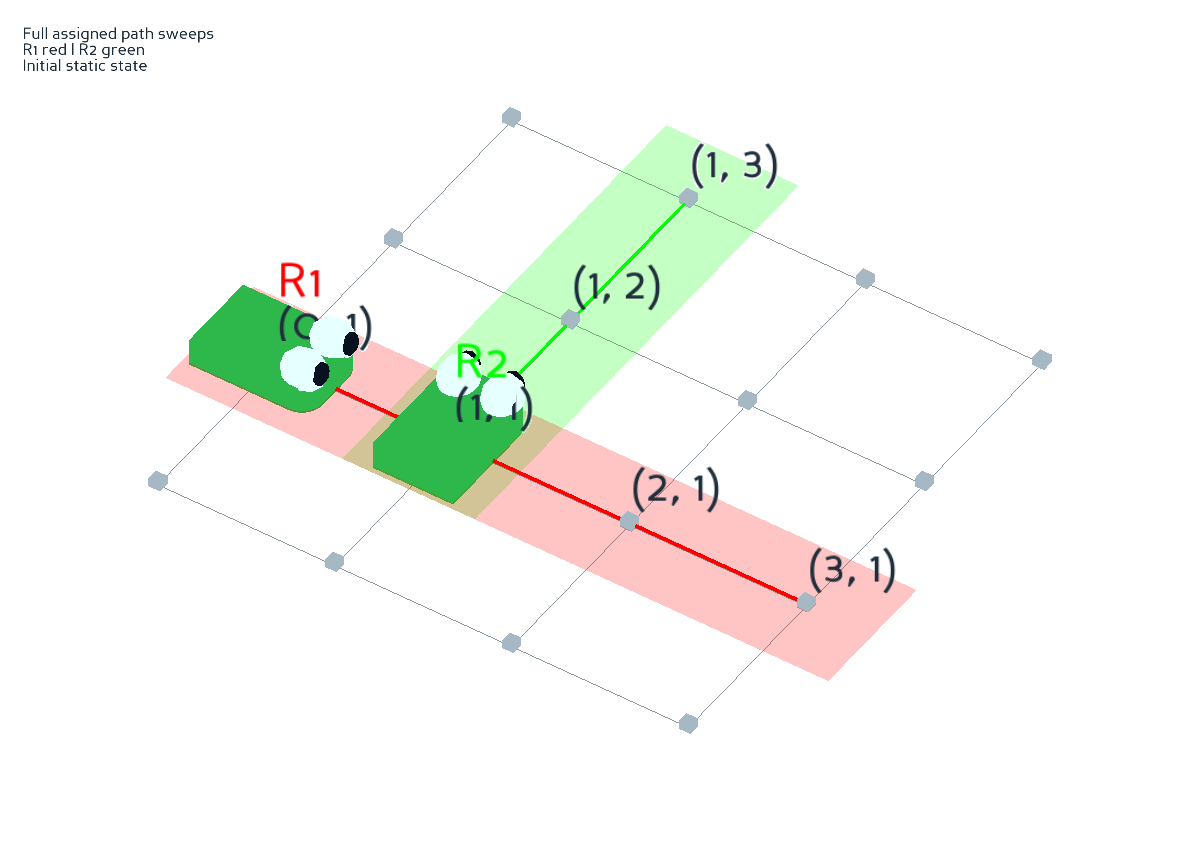
\includegraphics[height=2.6cm,keepaspectratio]{assets/paired_full_white.png}\par
{\scriptsize Full paths: overlapping sweeps.\par $S_1(P_1)\cap S_2(P_2)\ne\varnothing$.}
\end{column}
\begin{column}{.32\textwidth}\centering
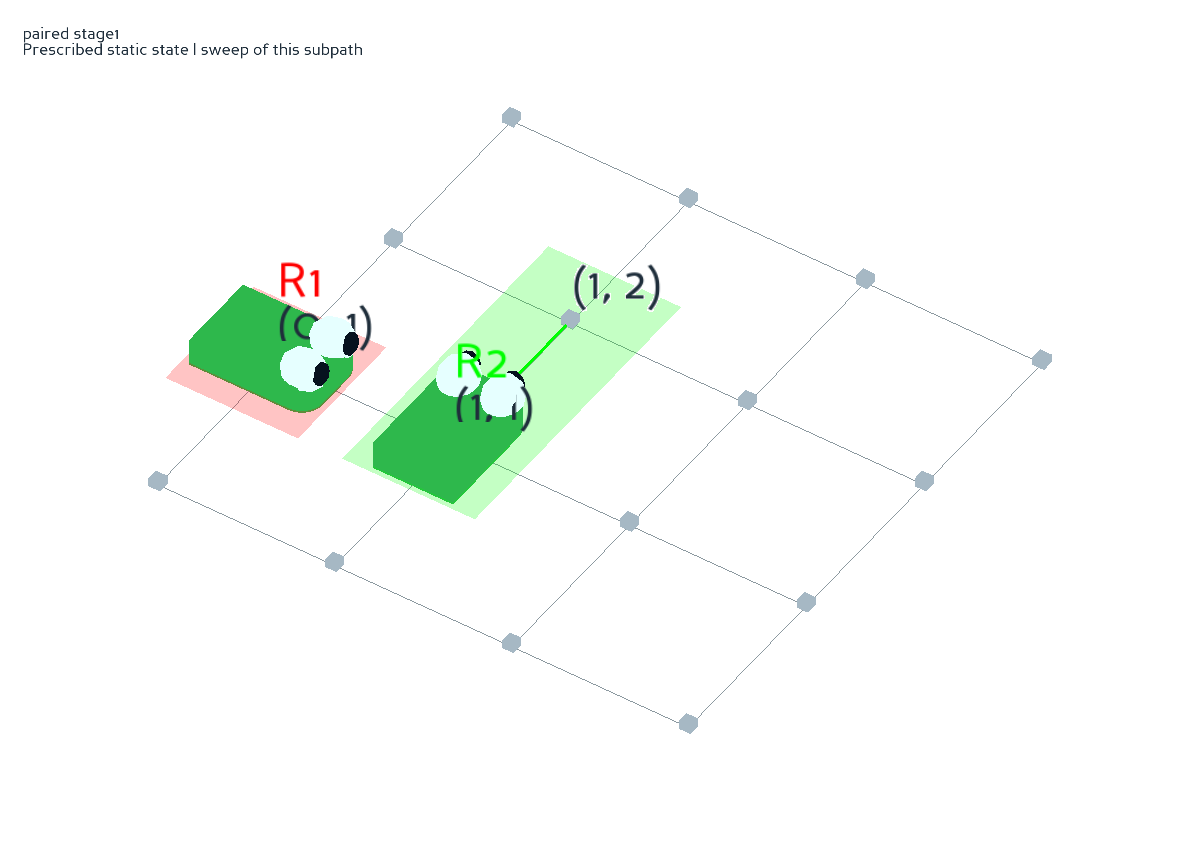
\includegraphics[height=2.6cm,keepaspectratio]{assets/paired_stage1_white.png}\par
{\scriptsize Pair 1: red waits; green moves up.\par The subpath sweeps are disjoint.}
\end{column}
\begin{column}{.32\textwidth}\centering
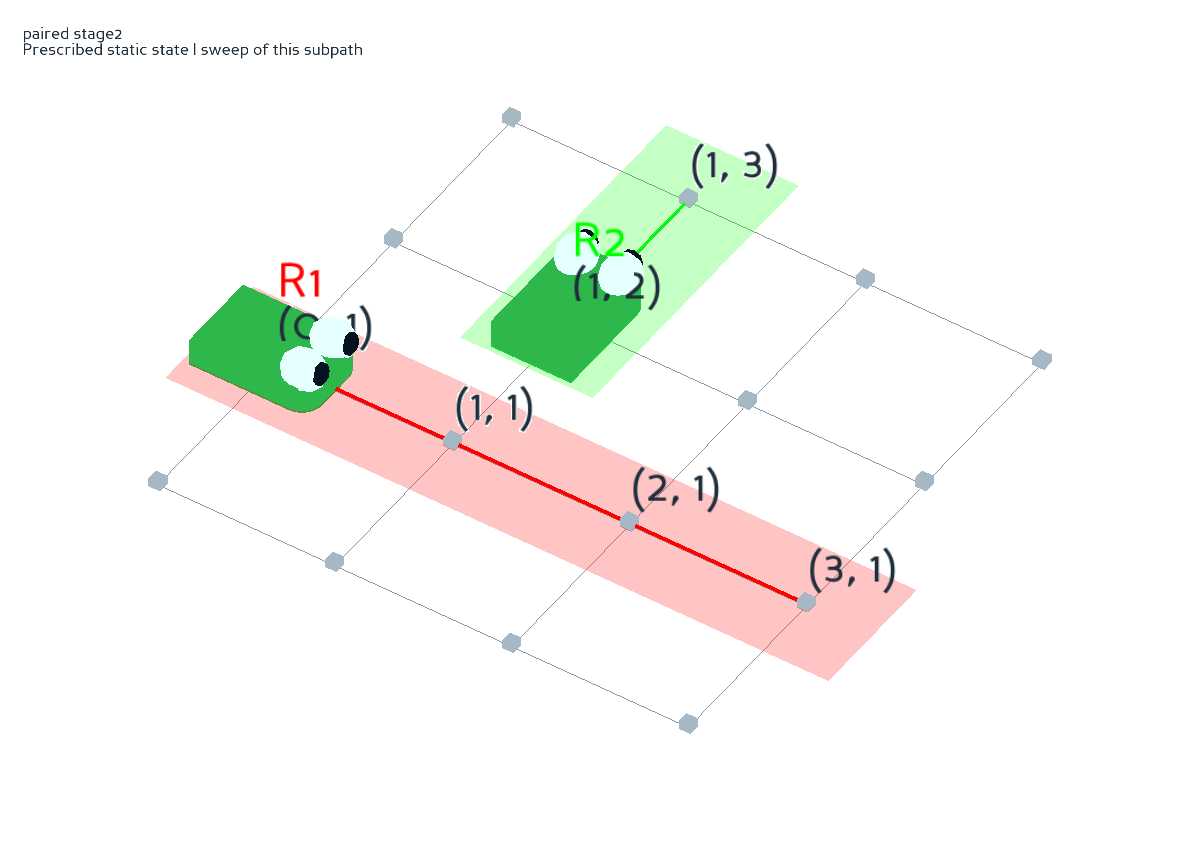
\includegraphics[height=2.6cm,keepaspectratio]{assets/paired_stage2_white.png}\par
{\scriptsize Pair 2: both follow their residual paths.\par The subpath sweeps are disjoint.}
\end{column}\end{columns}
\begin{equation}
\begin{aligned}
P_1^{(1)}&=[(0,1),(0,1)],& P_2^{(1)}&=[(1,1),(1,2)],\\
P_1^{(2)}&=[(0,1),(3,1)],& P_2^{(2)}&=[(1,2),(1,3)].
\end{aligned}
\tag{13}
\end{equation}
\small \textbf{Overlapping full sweeps do not imply infeasibility.} Each pair is interference-free, and concatenation recovers both original paths.
\par\smallskip\scriptsize Static views of the initial arrangement and two subpath pairs for Example 02\_09. Coordinates are grid point indices.
\end{frame}

\begin{frame}{Opposing paths: interference and the first safe pair}
\small The objects traverse the same horizontal aisle in opposite directions. Both starts and goals lie outside that aisle.
\par\smallskip
$P_1:(0,3)\to(0,2)\to(3,2)\to(3,3)$,\par
$P_2:(3,1)\to(3,2)\to(0,2)\to(0,1)$.
\begin{columns}[T]
\begin{column}{.49\textwidth}\centering
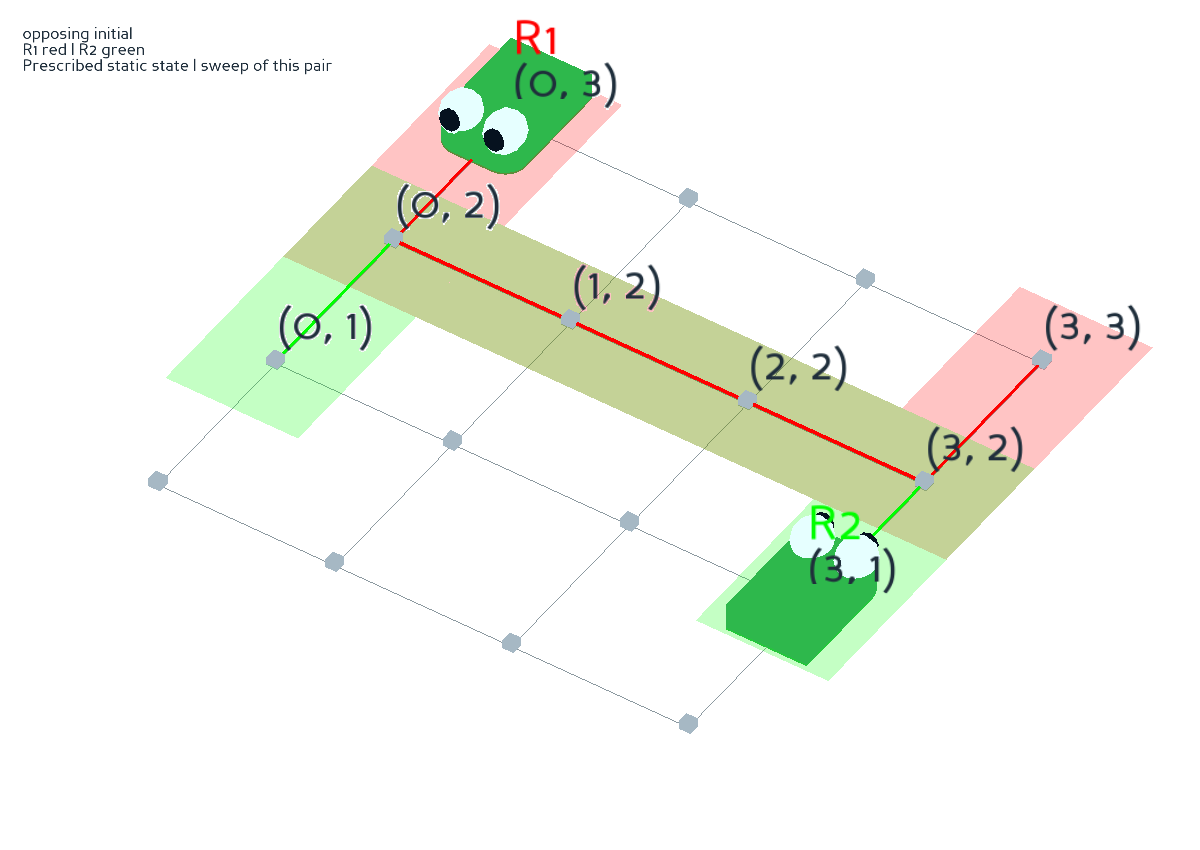
\includegraphics[height=2.8cm,keepaspectratio]{assets/opposing_initial_white.png}\par
{\scriptsize Initial full paths: red and green sweeps overlap.}
\end{column}\begin{column}{.49\textwidth}\centering
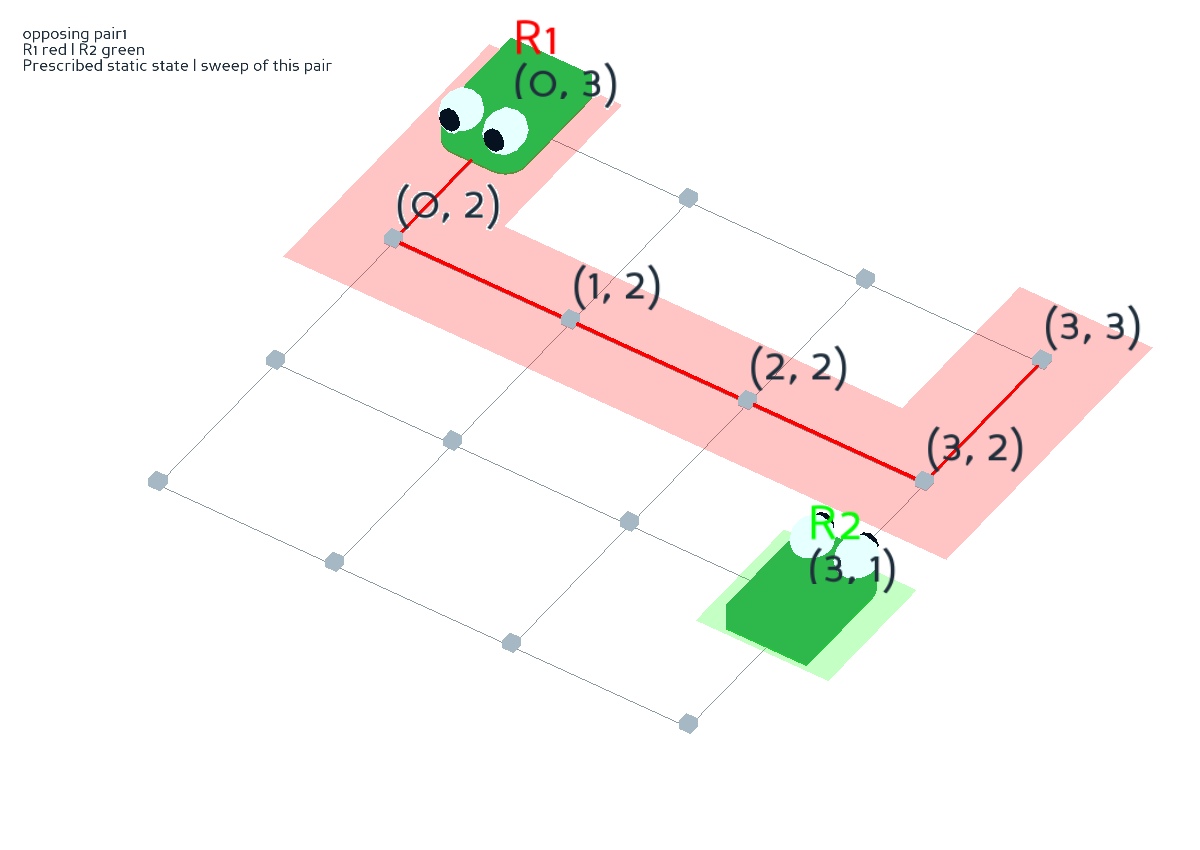
\includegraphics[height=2.8cm,keepaspectratio]{assets/opposing_pair1_white.png}\par
{\scriptsize Pair 1: green waits at its start; red completes its path.}
\end{column}\end{columns}

\begin{equation}
\begin{aligned}
&P_1^{(1)}=P_1,\qquad P_2^{(1)}=[(3,1),(3,1)],\\
&S_1(P_1^{(1)})\cap S_2(P_2^{(1)})=\varnothing.
\end{aligned}
\tag{13a}
\end{equation}
\small Green retains its square footprint at the start. That square is disjoint from red's full sweep, so red can cross the aisle and reach $(3,3)$.
\par\smallskip\scriptsize Static two-pair decomposition of Example 02\_07. Coordinates are grid point indices.
\end{frame}

\begin{frame}{Opposing paths: the second pair and completion}
\begin{columns}[T]
\begin{column}{.49\textwidth}\centering
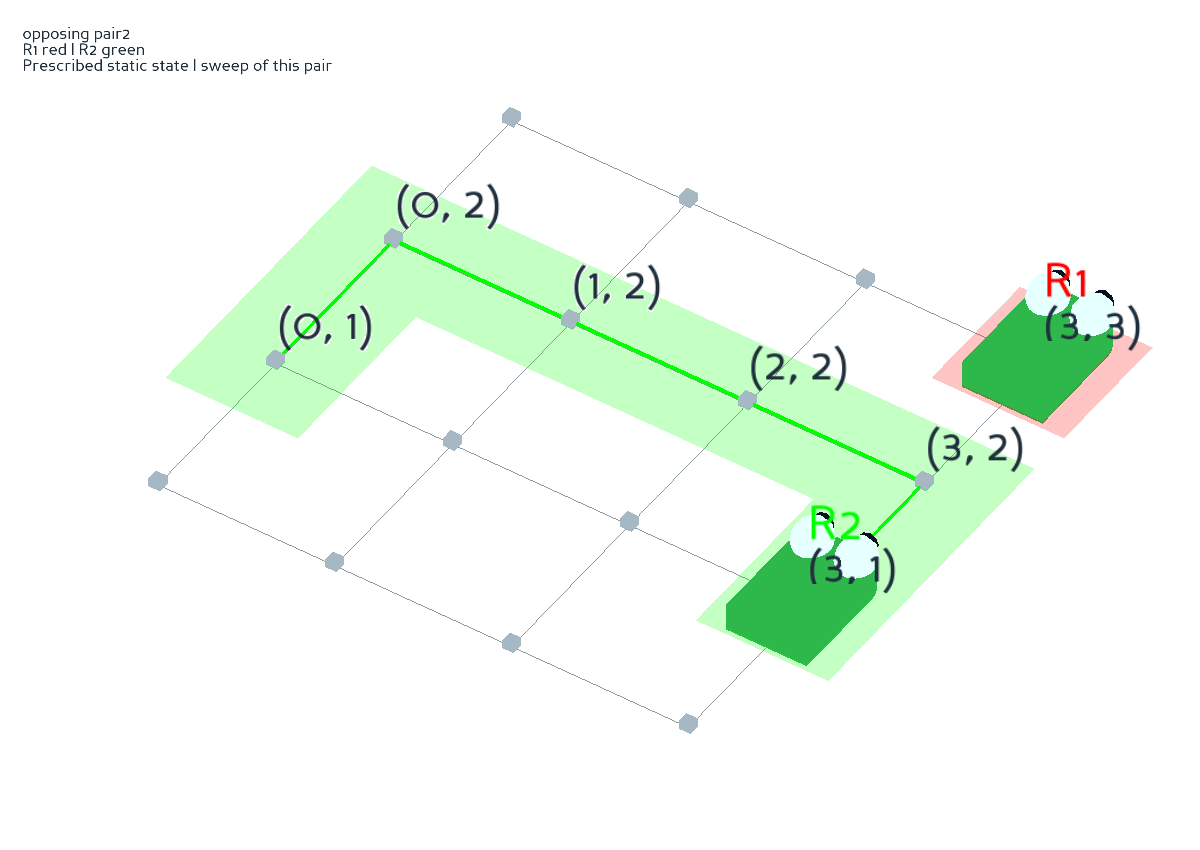
\includegraphics[height=2.8cm,keepaspectratio]{assets/opposing_pair2_white.png}\par
{\scriptsize Pair 2: red waits at its goal; green completes its path.}
\end{column}\begin{column}{.49\textwidth}\centering
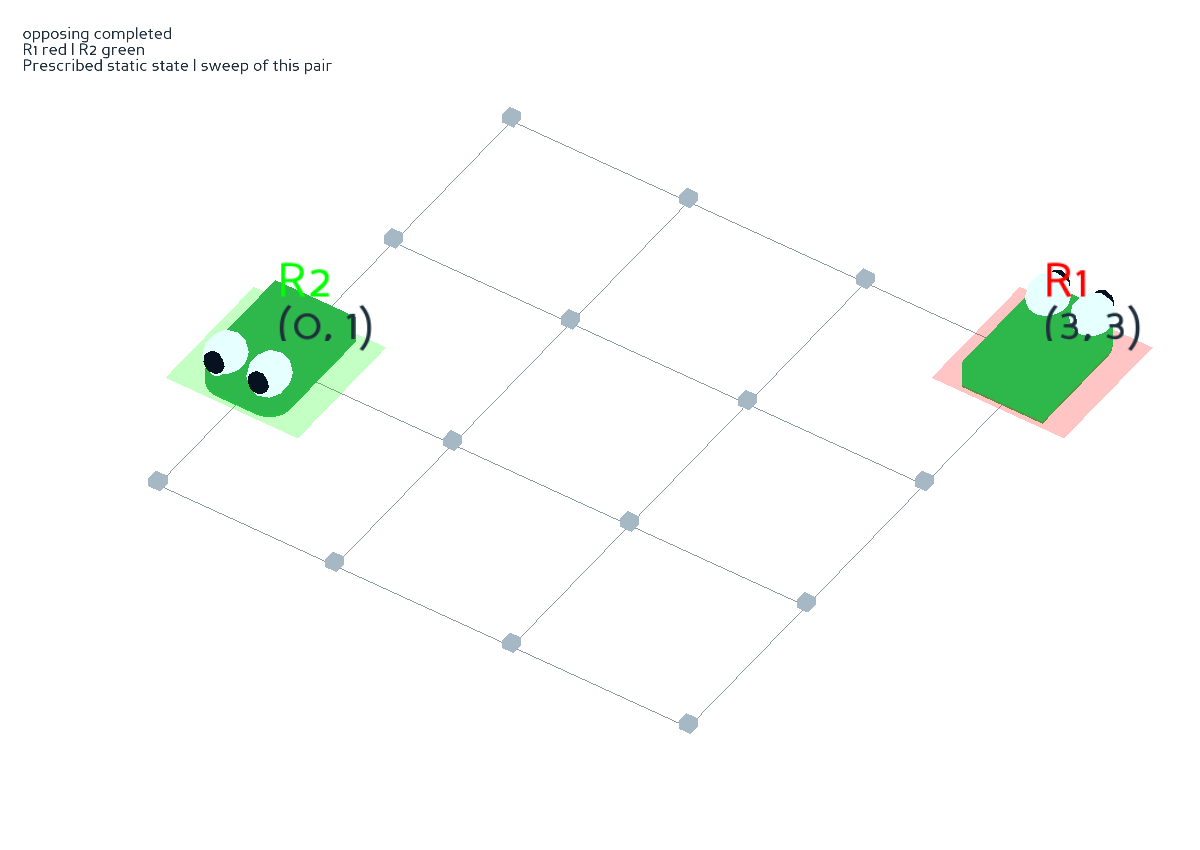
\includegraphics[height=2.8cm,keepaspectratio]{assets/opposing_completed_white.png}\par
{\scriptsize After both pairs: both objects have reached their goals.}
\end{column}\end{columns}

\begin{equation}
\begin{aligned}
&P_1^{(2)}=[(3,3),(3,3)],\qquad P_2^{(2)}=P_2,\\
&S_1(P_1^{(2)})\cap S_2(P_2^{(2)})=\varnothing.
\end{aligned}
\tag{13b}
\end{equation}
\small Red's goal footprint is disjoint from green's sweep. Green can cross the aisle in the opposite direction and reach $(0,1)$.
\medskip\par
\textbf{The full paths interfere, but each waiting-inclusive pair is interference-free.} Complete the first pair, then execute the second to finish both paths.
\par\smallskip\scriptsize Only subpath order and occupancy are used; numerical times and speeds are not assigned. These are prescribed static configurations, not a trace of automatic traffic control.
\end{frame}

\begin{frame}{Counterexample: opposing objects cannot complete a pairing}
\small Two objects start at opposite ends of one straight route and exchange endpoints. Paths are fixed; no side space or detour is used.
\begin{center}
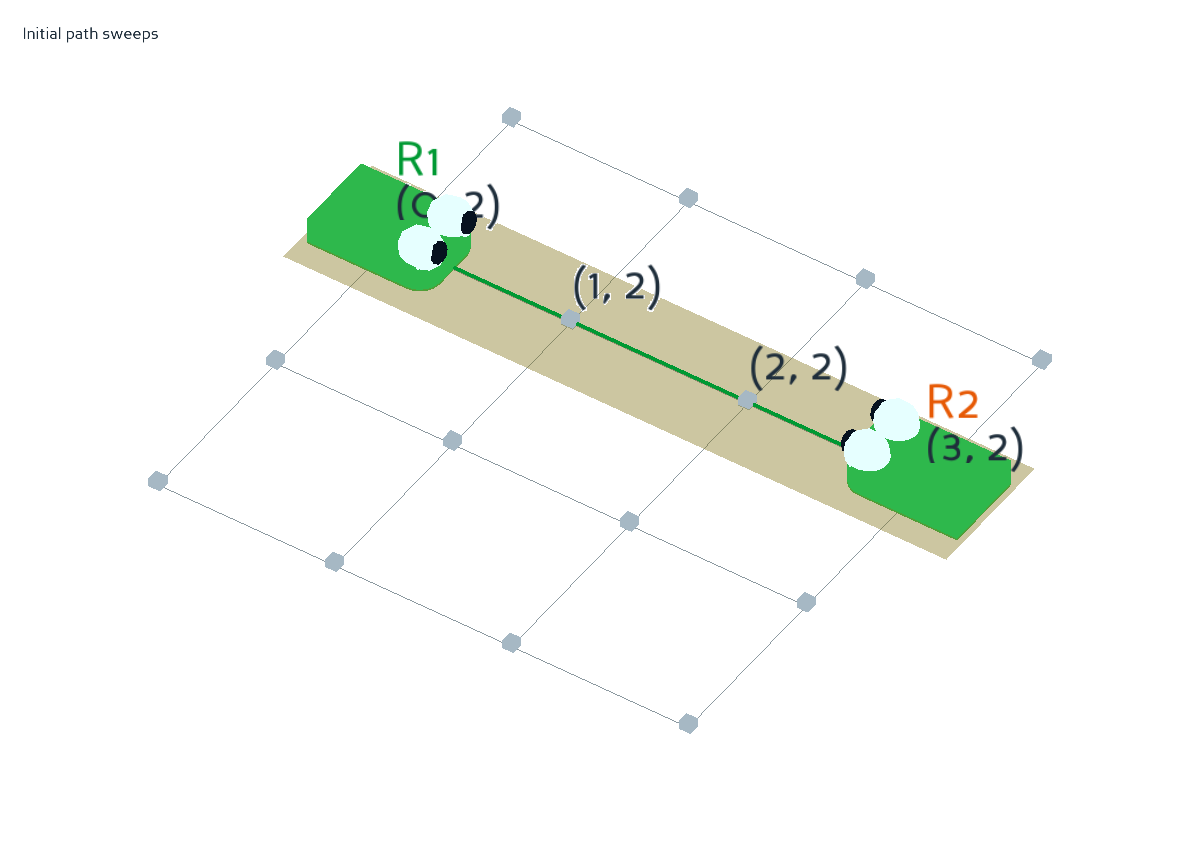
\includegraphics[height=3.0cm,keepaspectratio]{assets/p25_initial_white.png}\par
{\scriptsize $P_1:[(0,2),(3,2)]$,\quad $P_2:[(3,2),(0,2)]$. The full sweeps overlap.}
\end{center}
\small Both centers remain on the same line. Their left-to-right order is reversed between start and goal.
\begin{equation}
x_1^s<x_2^s,\qquad x_1^e>x_2^e.
\tag{13c}
\end{equation}
\small Reversing that order continuously requires the bodies to meet. Neither waiting nor changing the first mover can therefore produce a \textbf{finite interference-free pairing that completes both paths}.
\par\smallskip{\tiny\texttt{\detokenize{python -m examples.RMFS.Tests.02_05_RobotPath_OppositeDirection_Collision --white-background}}}
\end{frame}

\begin{frame}{Theorem 1: safe completion by disjoint-sweep pairing}
\textbf{Theorem 1.} Suppose the two full paths are concatenations of finitely many interference-free subpath pairs, and each pair takes finite time to execute. Then \textbf{executing those pairs in order completes both paths in finite time without collision}.
\medskip\par
\textbf{Proof.} The two sweeps in each pair are disjoint. Each object's occupancy, while moving or waiting at the endpoint, remains within its own sweep. Thus that pair executes without collision.
\medskip\par
Start the next pair only after both components of the current pair finish. Consequently the full execution is collision-free. The number of pairs and each pair's duration are finite, so their total duration is finite.
\medskip\par
Concatenating the subpaths recovers both full paths. Hence both objects reach their respective goals \textbf{in finite time}.\hfill$\square$
\end{frame}

\begin{frame}{Applying Theorem 1 to three moving objects}
Decompose all three paths into a \textbf{common number $m$ of stages}, with one triple of subpaths at each stage.
\[
\left(P_1^{(k)},P_2^{(k)},P_3^{(k)}\right),\qquad k=1,\ldots,m.
\]
Every pair of objects must have disjoint sweeps within each triple.
\begin{equation}
S_r(P_r^{(k)})\cap S_s(P_s^{(k)})=\varnothing,
\quad 1\le r<s\le3,\quad k=1,\ldots,m.
\tag{14}
\end{equation}
\textbf{Corollary.} If each triple has a finite execution duration, executing the triples in order completes all three paths in finite time without collision.
\medskip\par
\small \textbf{Reason:} apply Theorem 1's sweep-containment argument to all three object pairs at the same stage $k$. No two bodies can meet. The finite sequence of triples completes the full paths.
\medskip\par
\textbf{Important:} separately feasible pairwise orders are insufficient. All three objects need \textbf{one common stage decomposition}.
\end{frame}

\begin{frame}{Feasible example: the initial full sweeps overlap}
\begin{columns}[T]
\begin{column}{.51\textwidth}\centering
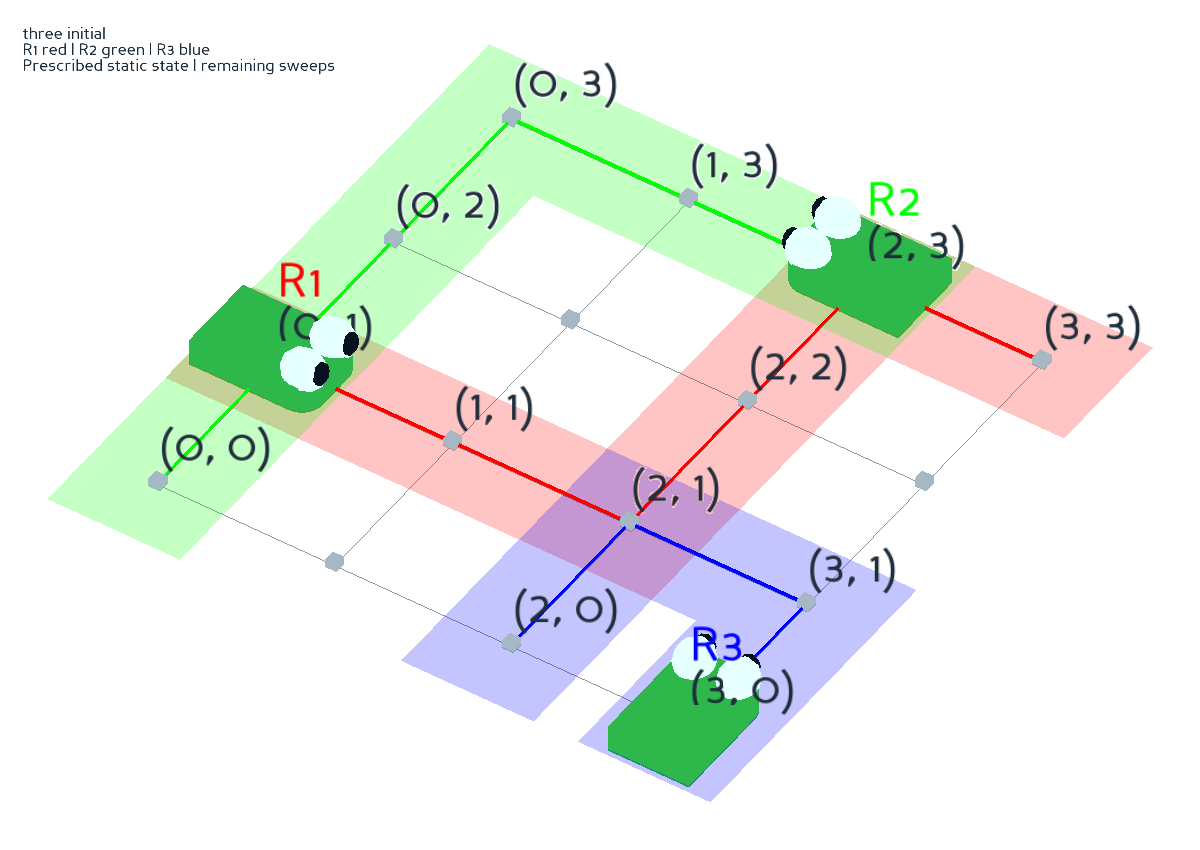
\includegraphics[height=3.65cm,keepaspectratio]{assets/three_initial_white.png}
\end{column}\begin{column}{.47\textwidth}\small
\textbf{Three fixed paths in Example 03\_04}
\[
\begin{aligned}
P_1:\ &(0,1)\to(2,1)\\
&\to(2,3)\to(3,3),\\
P_2:\ &(2,3)\to(0,3)\to(0,0),\\
P_3:\ &(3,0)\to(3,1)\\
&\to(2,1)\to(2,0).
\end{aligned}
\]
Red overlaps both green and blue; green and blue are disjoint. The next three triples account for all three objects together.
\end{column}\end{columns}
\small Red, green and blue denote objects 1, 2 and 3 throughout. Coordinates are grid point indices. Each stage view shows only that stage's subpath sweeps.
\par\smallskip{\tiny\texttt{\detokenize{python -m examples.RMFS.Tests.03_04_RobotPath_SweepInterference --white-background}}}
\end{frame}

\begin{frame}{Triple 1: red and green wait while blue clears}
\begin{columns}[T]
\begin{column}{.49\textwidth}\centering
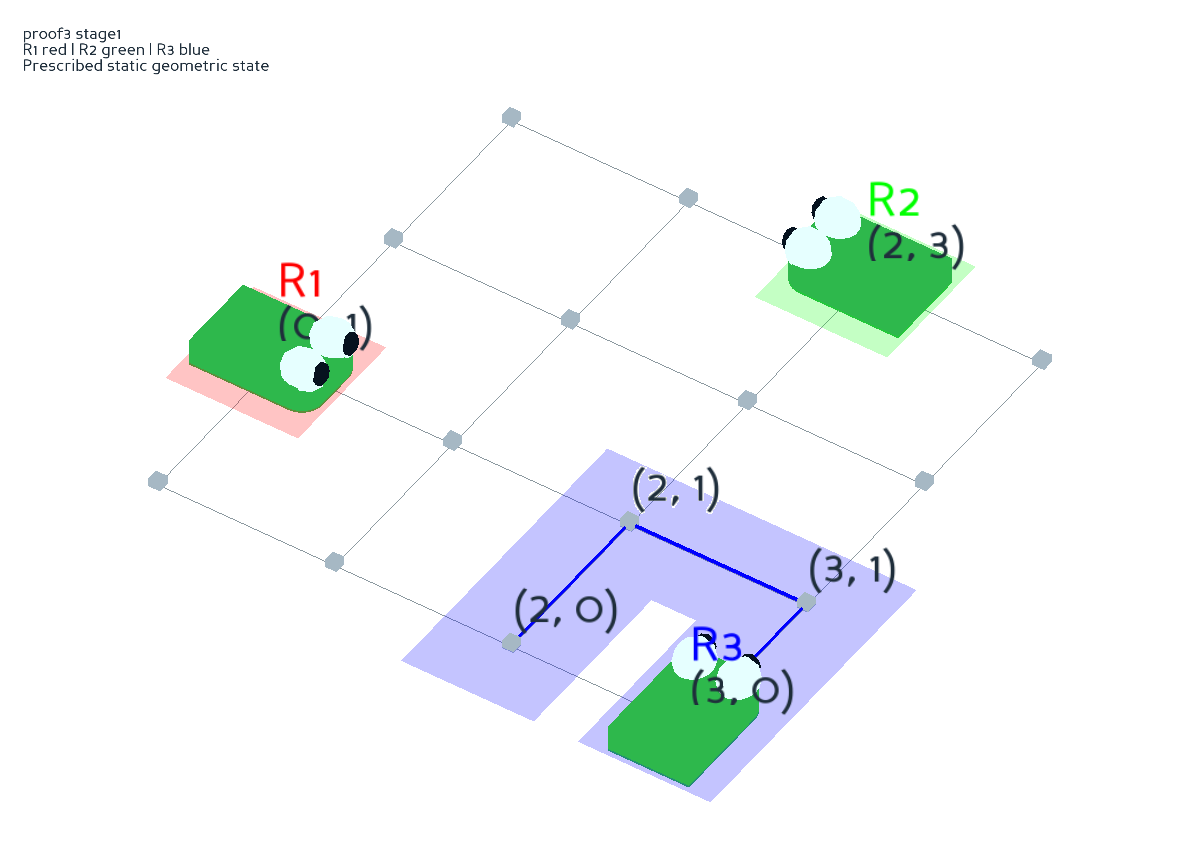
\includegraphics[height=2.65cm,keepaspectratio]{assets/proof3_stage1_white.png}\par{\scriptsize Current triple: two point paths and blue's full path.}
\end{column}\begin{column}{.49\textwidth}\centering
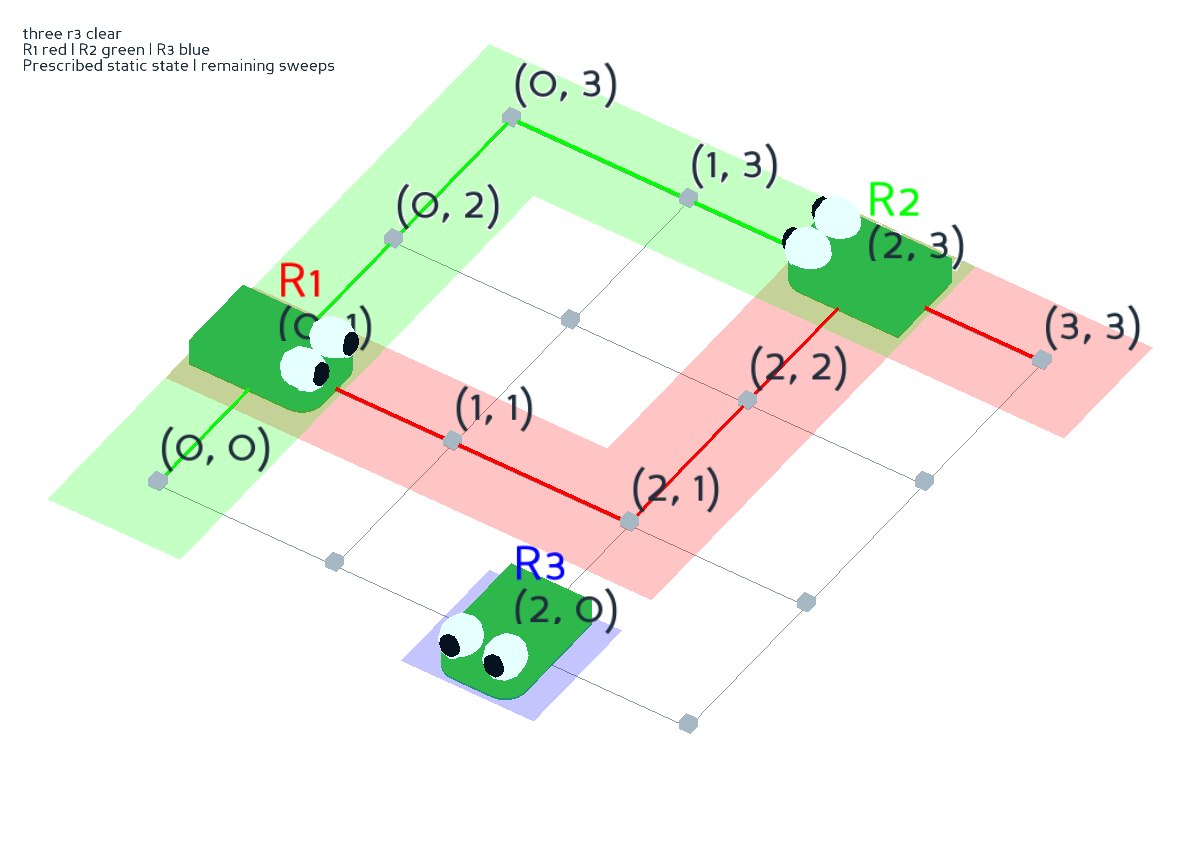
\includegraphics[height=2.65cm,keepaspectratio]{assets/three_r3_clear_white.png}\par{\scriptsize Residual paths: red and green still interfere.}
\end{column}\end{columns}

\begin{equation}
\begin{aligned}
P_1^{(1)}&=[(0,1),(0,1)],\\
P_2^{(1)}&=[(2,3),(2,3)],\qquad P_3^{(1)}=P_3.
\end{aligned}
\tag{15}
\end{equation}
\small Blue's sweep is disjoint from the current red and green footprints. The two waiting footprints are also separated, so all three pairs are interference-free.
\medskip\par
Blue reaches $(2,0)$ and retains only its footprint. Red and green still have overlapping residual sweeps, handled by the next triples.
\end{frame}

\begin{frame}{Triples 2 and 3: completing the remaining subpaths}
\begin{columns}[T]
\begin{column}{.49\textwidth}\centering
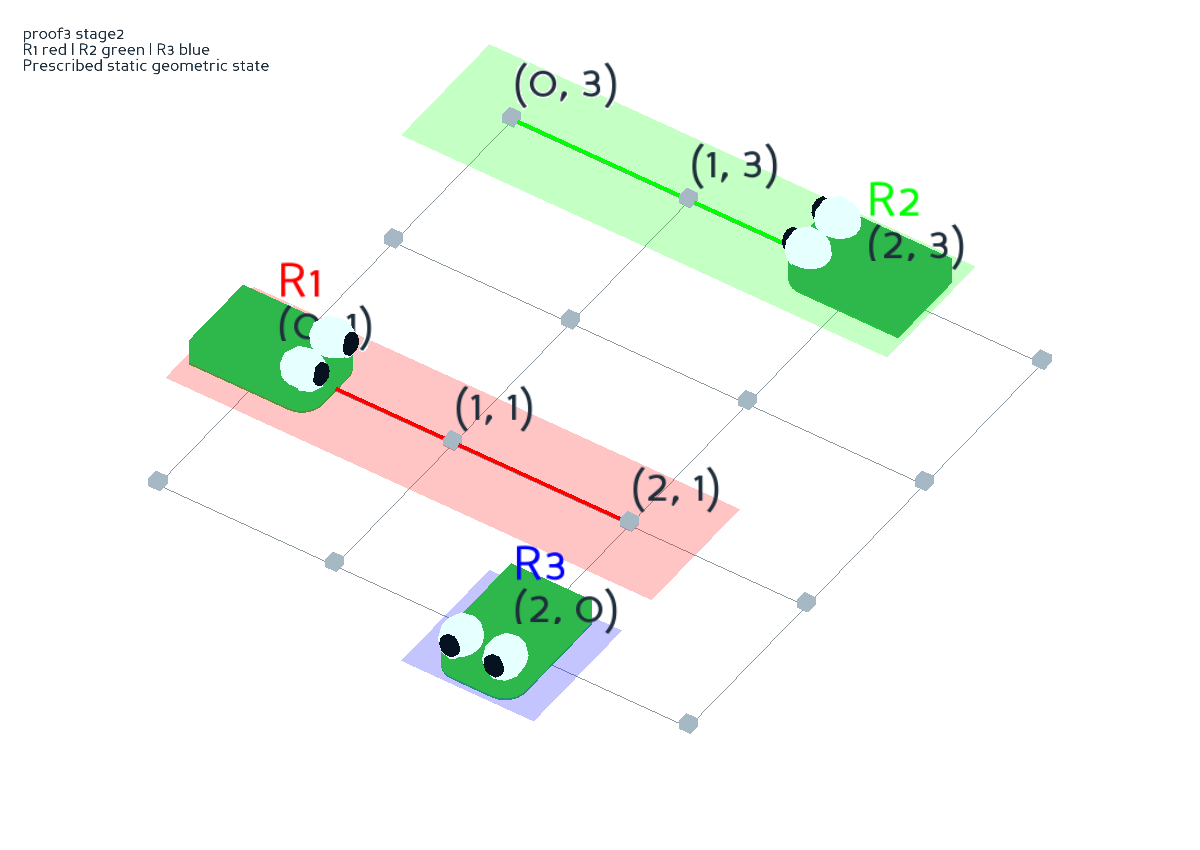
\includegraphics[height=2.65cm,keepaspectratio]{assets/proof3_stage2_white.png}\par{\scriptsize Triple 2: red and green advance; blue waits.}
\end{column}\begin{column}{.49\textwidth}\centering
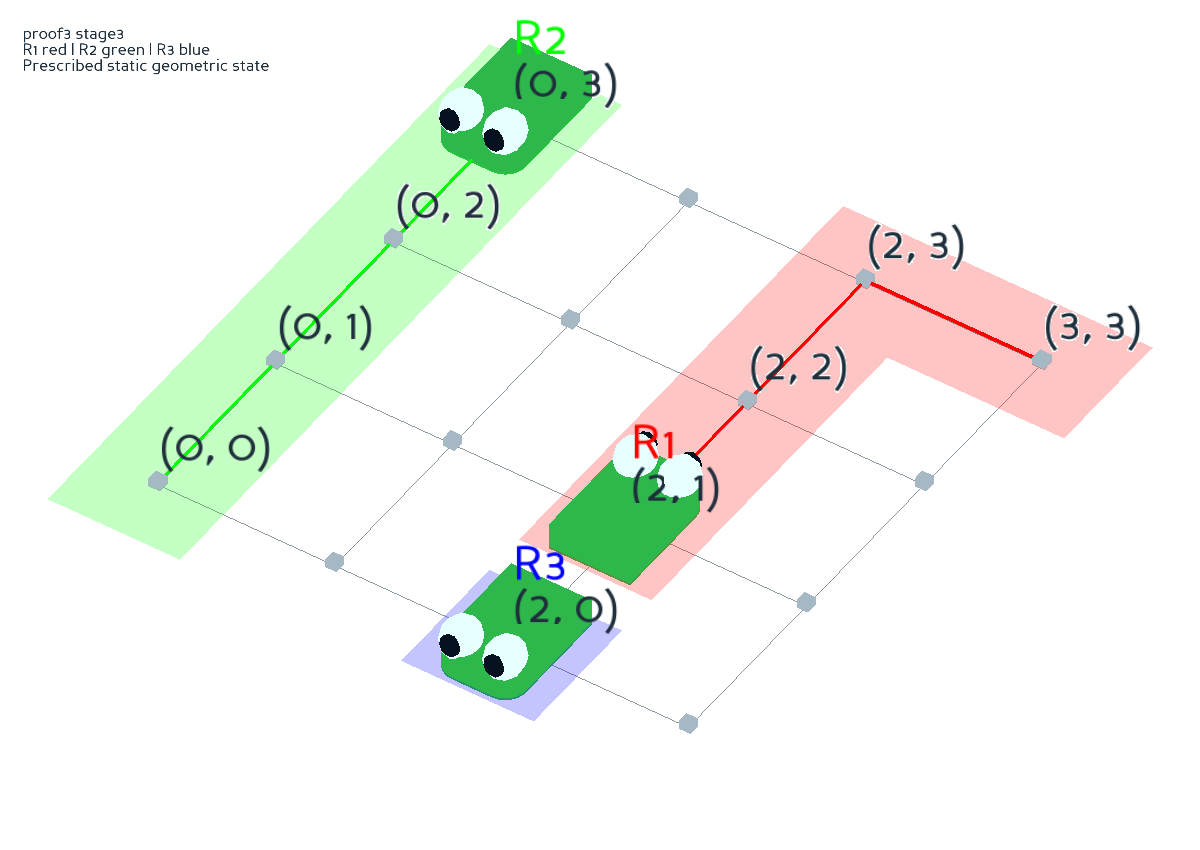
\includegraphics[height=2.65cm,keepaspectratio]{assets/proof3_stage3_white.png}\par{\scriptsize Triple 3: red and green finish; blue waits.}
\end{column}\end{columns}

\begin{equation}
\begin{aligned}
(P_1^{(2)},P_2^{(2)})&=\bigl([(0,1),(2,1)],[(2,3),(0,3)]\bigr),\\
(P_1^{(3)},P_2^{(3)})&=\bigl([(2,1),(2,3),(3,3)],[(0,3),(0,0)]\bigr),\\
P_3^{(2)}=P_3^{(3)}&=[(2,0),(2,0)].
\end{aligned}
\tag{16}
\end{equation}
\small In triple 2, the two horizontal sweeps and blue's footprint are disjoint. Triple 3 likewise separates the left and right sweeps from blue's footprint.
\par\smallskip\scriptsize Both triples satisfy all three pairwise conditions in Eq. (14). Numerical times and relative speeds are not specified.
\end{frame}

\begin{frame}{Completion check: all three triples satisfy Theorem 1}
\begin{columns}[T]
\begin{column}{.48\textwidth}\centering
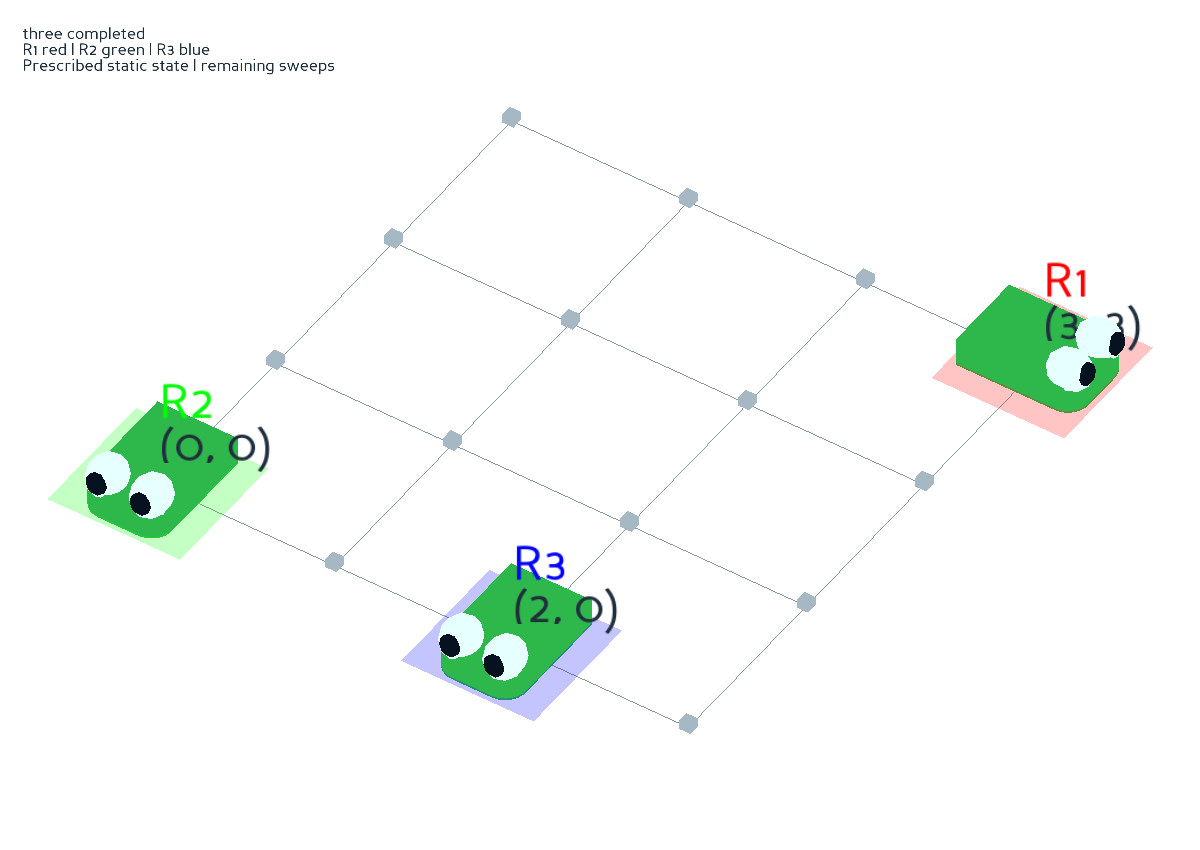
\includegraphics[height=3.35cm,keepaspectratio]{assets/three_completed_white.png}
\end{column}\begin{column}{.50\textwidth}\small
\textbf{Pairwise sweep intersections in each triple}
\begin{center}
\begin{tabular}{cccc}\toprule
Triple & 1--2 & 1--3 & 2--3\\\midrule
1 & $\varnothing$ & $\varnothing$ & $\varnothing$\\
2 & $\varnothing$ & $\varnothing$ & $\varnothing$\\
3 & $\varnothing$ & $\varnothing$ & $\varnothing$\\\bottomrule
\end{tabular}
\end{center}
Concatenating each object's three subpaths recovers its original path. All three common triples, including waits, are interference-free. Finite execution of each triple therefore completes all three paths.
\end{column}\end{columns}
\begin{equation}
\text{Goal grid points:}\quad p_1^e=(3,3),\qquad p_2^e=(0,0),\qquad p_3^e=(2,0).
\tag{17}
\end{equation}
\small This is a \textbf{constructive feasibility witness}, not a claim of optimality or feasibility for arbitrary three-object paths. The table was checked using fixed rectangular sweeps.
\end{frame}

\begin{frame}{Infeasible example: three paths through one center}
\begin{columns}[T]
\begin{column}{.49\textwidth}\centering
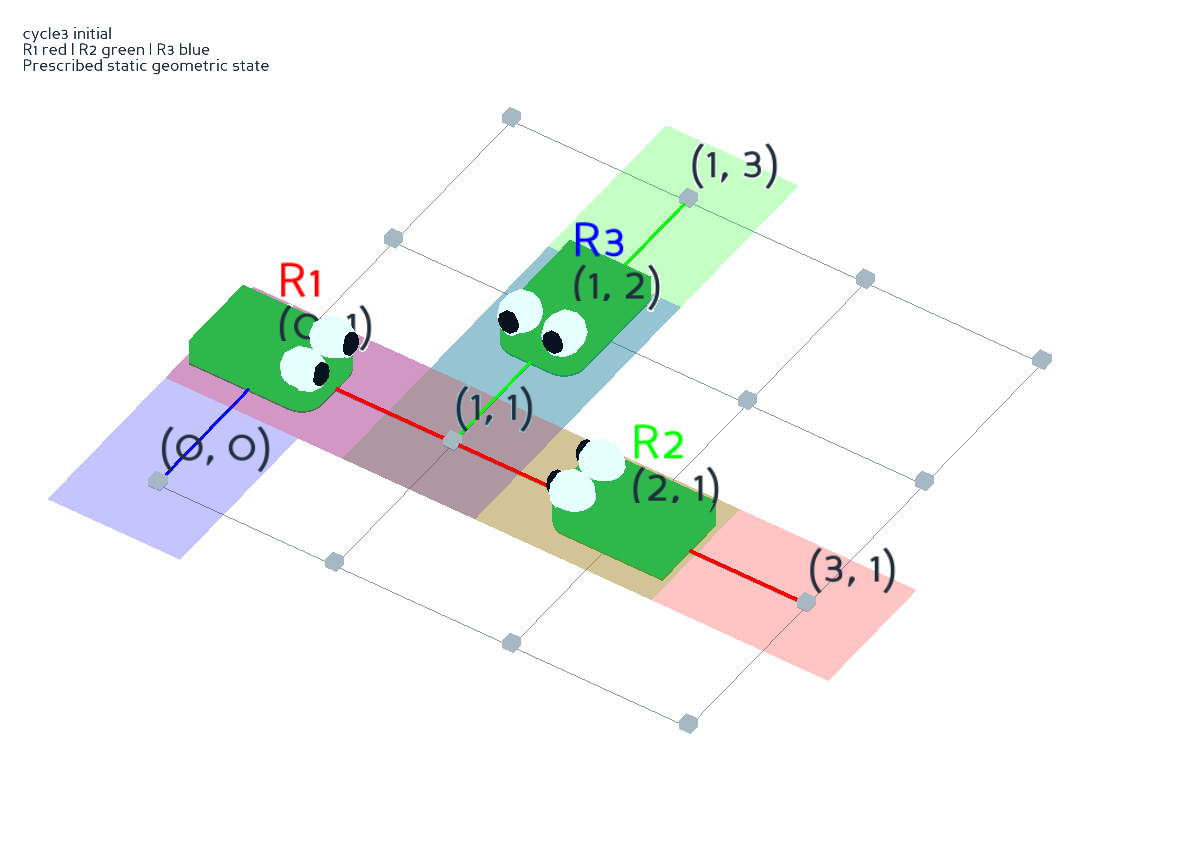
\includegraphics[height=3.65cm,keepaspectratio]{assets/cycle3_initial_white.png}
\end{column}\begin{column}{.49\textwidth}\small
\textbf{Example 03\_06}
\[
\begin{aligned}
P_1:\ &(0,1)\to(1,1)\\
&\to(2,1)\to(3,1),\\
P_2:\ &(2,1)\to(1,1)\\
&\to(1,2)\to(1,3),\\
P_3:\ &(1,2)\to(1,1)\\
&\to(0,1)\to(0,0).
\end{aligned}
\]
Each object must pass through $(1,1)$ and another object's start to reach its goal.
\end{column}\end{columns}
\small \textbf{Allowed execution:} forward motion and waiting on fixed paths; subpath endpoints are grid points. No detours or reverse motion. Grid spacing is 2 m; the square footprint has side length 1.5 m.
\par\smallskip{\tiny\texttt{\detokenize{python -m examples.RMFS.Tests.03_06_RobotPath_ThreeWay_CyclicWait --white-background}}}
\end{frame}

\begin{frame}{Why no complete interference-free tuple sequence exists}
\begin{columns}[T]
\begin{column}{.32\textwidth}\centering
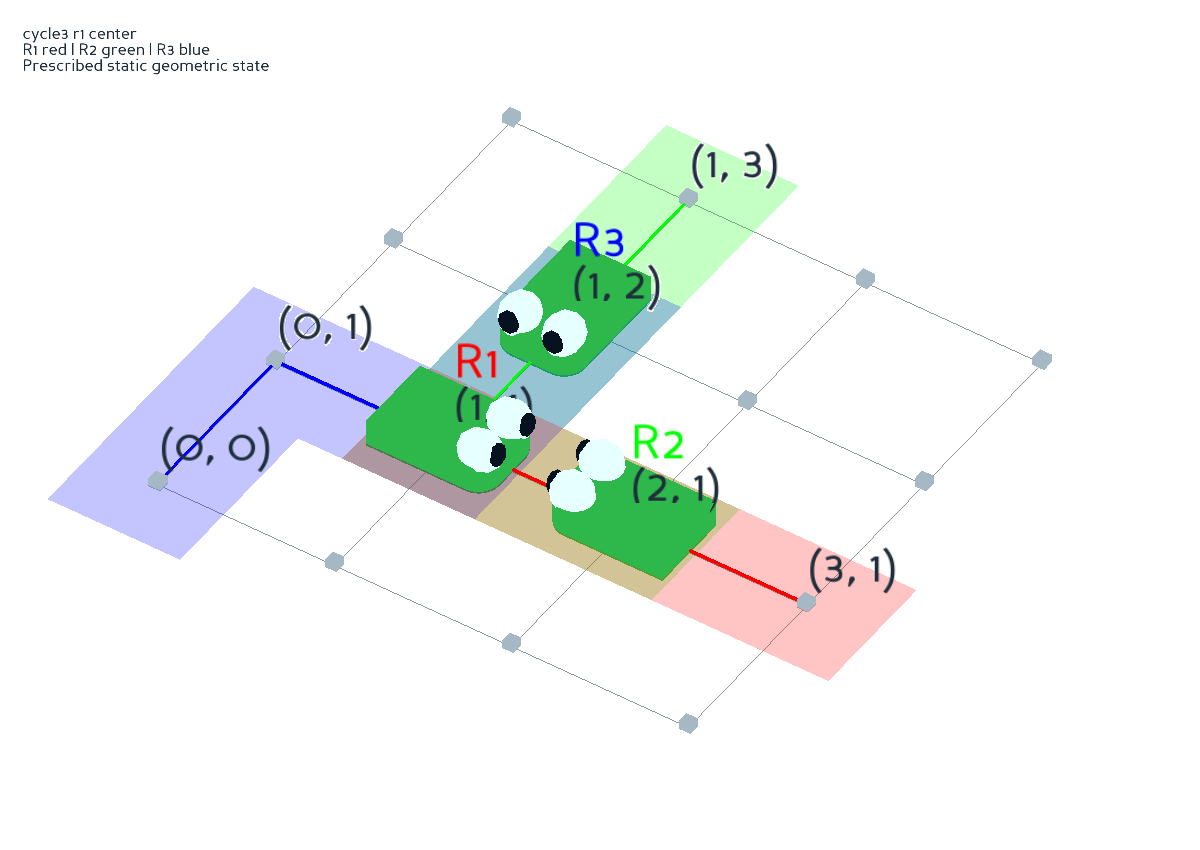
\includegraphics[height=2.1cm,keepaspectratio]{assets/cycle3_r1_center_white.png}\par{\scriptsize Red enters the center first.}
\end{column}\begin{column}{.32\textwidth}\centering
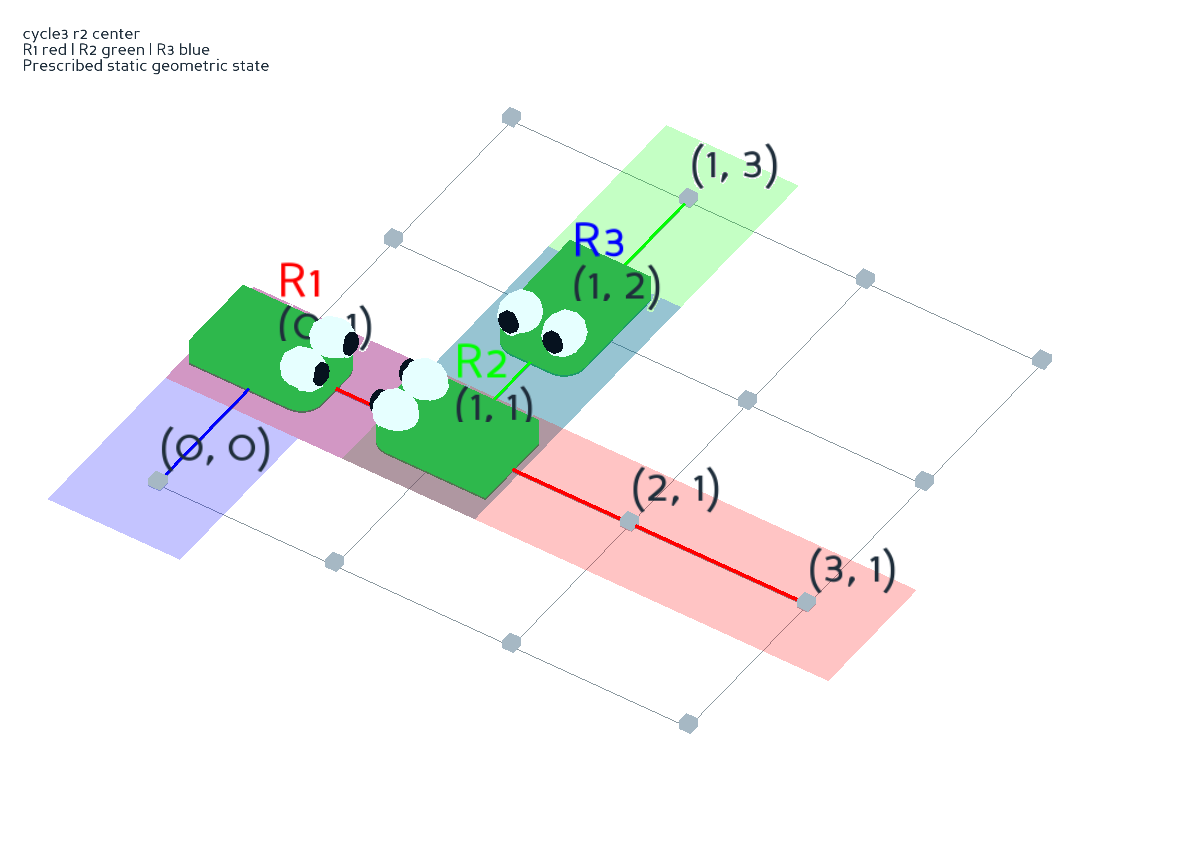
\includegraphics[height=2.1cm,keepaspectratio]{assets/cycle3_r2_center_white.png}\par{\scriptsize Green enters the center first.}
\end{column}\begin{column}{.32\textwidth}\centering
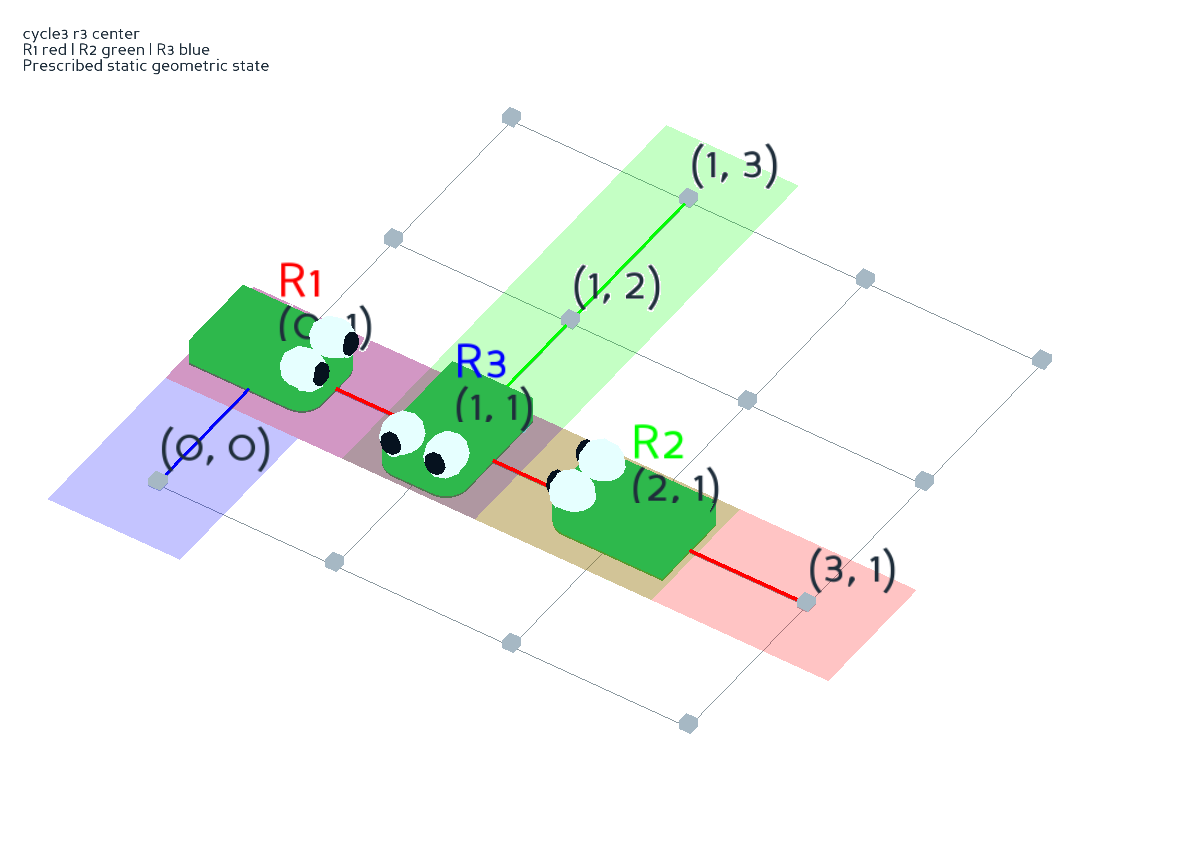
\includegraphics[height=2.1cm,keepaspectratio]{assets/cycle3_r3_center_white.png}\par{\scriptsize Blue enters the center first.}
\end{column}\end{columns}
\small In the first tuple with any forward progress, two moving objects would both sweep the center. Hence only one object can advance first.
\medskip\par
If red enters, its next point $(2,1)$ is occupied by green. The next point for green and blue, $(1,1)$, is occupied by red. Choosing another first mover gives the same obstruction.
\begin{equation}
(0,0,0)\longrightarrow
(1,0,0)\ \text{or}\ (0,1,0)\ \text{or}\ (0,0,1).
\tag{18}
\end{equation}
\scriptsize Entries are waypoint indices: start 0, center 1, goal 3. Enumerating allowed subpath tuples reaches only the initial state and these three states, never $(3,3,3)$. In-place rotation does not change the square footprint.
\end{frame}








% Discussion record: audited terminology, tree structure and four operations.


\begin{frame}{Extended interference subpaths: finite boundary choices}
\small
For a continuous simple path $P_i:[0,1]\to Q_i$, suppose the progress values that
interfere with the other object's full sweep form one nonempty interval $[a,b]$.
The parameter denotes path order, not time.
\begin{equation}
 C_{i\mid j}=\{u:B_i(u)\cap S(P_j)\ne\varnothing\}=[a,b].\tag{24}
\end{equation}
Let $D_i$ be the parameters of a finite set of selected points on the path. If both
sets below are nonempty, choose the nearest interference-free points before and after the interval.
\begin{equation}
 a^- =\max\{d\in D_i:d<a\},\qquad
 b^+ =\min\{d\in D_i:d>b\},\qquad
 \widehat I_{i\mid j}=P_i|_{[a^-,b^+]}.\tag{25}
\end{equation}
\begin{center}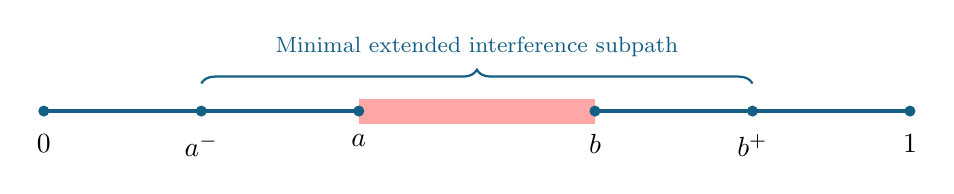
\begin{tikzpicture}[x=1cm,y=1cm]
\draw[very thick,accent] (0,0)--(11,0);
\draw[line width=9pt,red!35] (4,0)--(7,0);
\draw[thick,accent,decorate,decoration={brace,amplitude=5pt}] (2,0.35)--(9,0.35)
 node[midway,above=6pt]{\footnotesize Minimal extended interference subpath};
\foreach \x/\lab in {0/0,2/{a^-},4/a,7/b,9/{b^+},11/1}
 {\fill[accent] (\x,0) circle(2pt);\node[below=5pt] at (\x,0) {$\lab$};}
\end{tikzpicture}\end{center}
\footnotesize Both endpoint footprints are disjoint from the other object's full sweep.
For fixed $D_i$, this is the unique minimal extension under path inclusion among
extensions containing the interference subpath with interference-free selected endpoints.
If either candidate set is empty, this two-sided extension is undefined; that alone does not prove infeasibility.
\end{frame}

\begin{frame}{Why finitely many points? A minimum may not exist}
\small
If stopping is allowed anywhere on the continuous path and the boundaries $a,b$ themselves interfere,
any interference-free choices $u<a$, $v>b$ can be moved closer to those boundaries.
\begin{equation}
 u<\frac{u+a}{2}<a,\qquad
 b<\frac{b+v}{2}<v.\tag{26}
\end{equation}
Thus extensions with interference-free endpoints may exist while
\textbf{a shortest such extension does not exist.}
A limiting interference boundary is not an actual interference-free stopping point.
\begin{center}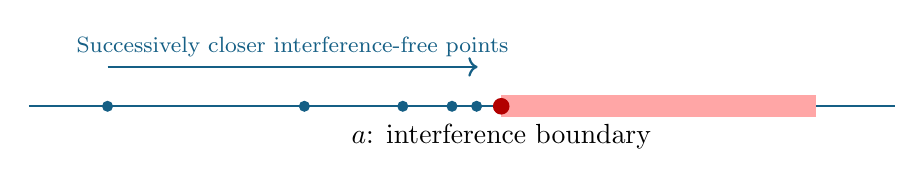
\begin{tikzpicture}[x=1cm,y=1cm]
\draw[thick,accent] (0,0)--(11,0);
\draw[line width=8pt,red!35] (6,0)--(10,0);
\foreach \x in {1,3.5,4.75,5.375,5.6875}
 {\fill[accent] (\x,0) circle(2pt);}
\fill[red!70!black] (6,0) circle(3pt);
\node[below] at (6,-.1) {$a$: interference boundary};
\draw[->,accent,thick] (1,.5)--(5.7,.5)
 node[midway,above]{\footnotesize Successively closer interference-free points};
\end{tikzpicture}\end{center}
\textbf{A finite point set discretizes the boundary choices.}
When both candidate sets exist, their maximum and minimum determine the minimal extension.
\par\medskip\footnotesize
This explains the mathematical role of a finite point set on the path. Physical stopping feasibility and safety margins
are separate requirements. Here the argument is geometric; a necessary-and-sufficient criterion for full completion
has not been established.
\end{frame}

\begin{frame}{Constructing paired paths: initial and terminal subpaths}
\small
Temporarily set sweeps aside and consider the path regions of two continuous simple paths
$P_i:[0,1]\to Q$, $i=1,2$. Define their interference parameter sets by
\begin{equation}
 C_i=\{u\in[0,1]:P_i(u)\in\operatorname{im}P_j\},\qquad j\ne i
 \tag{27}
\end{equation}
Here $\operatorname{im}P_j$ is the other path's entire image.
For nonempty $C_i$, let $a_i=\min C_i$ and $b_i=\max C_i$.
Define
\begin{equation}
 P_i^-=P_i|_{[0,a_i)},\qquad P_i^+=P_i|_{(b_i,1]}
 \tag{28}
\end{equation}
as the \textbf{initial subpath} and \textbf{terminal subpath}, respectively.
Even with several interference components, use the first and last boundaries of the entire interference set.
\begin{center}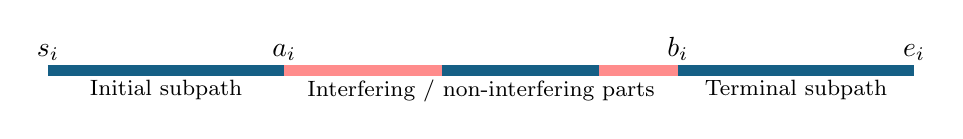
\begin{tikzpicture}[x=1cm,y=1cm]
\draw[line width=4pt,accent] (0,0)--(3,0);
\draw[line width=4pt,red!45] (3,0)--(5,0);
\draw[line width=4pt,accent] (5,0)--(7,0);
\draw[line width=4pt,red!45] (7,0)--(8,0);
\draw[line width=4pt,accent] (8,0)--(11,0);
\node[below] at (1.5,0){\footnotesize Initial subpath};
\node[below] at (5.5,0){\footnotesize Interfering / non-interfering parts};
\node[below] at (9.5,0){\footnotesize Terminal subpath};
\node[above] at (0,0){$s_i$};\node[above] at (3,0){$a_i$};
\node[above] at (8,0){$b_i$};\node[above] at (11,0){$e_i$};
\end{tikzpicture}\end{center}
\footnotesize If there is no interference, the two full paths are already disjoint.
Lengths in this schematic are conceptual, not execution times.
\end{frame}

\begin{frame}{Wait duplication and sweep merging}
\small
A \textbf{subpath sweep} is the swept region of a subpath. A \textbf{point sweep} is the footprint of a point path.
The constituent sweeps retain their path order.
\begin{center}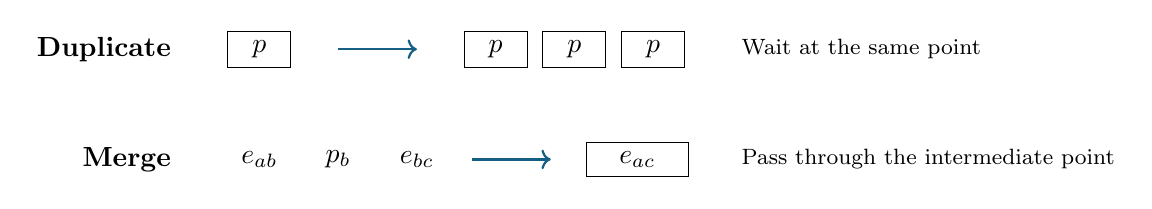
\begin{tikzpicture}[x=1cm,y=1cm]
\node[left] at (0,1.4){\textbf{Duplicate}};
\node[draw,minimum width=.8cm] at (1,1.4){$p$};
\draw[->,thick,accent] (2,1.4)--(3,1.4);
\foreach \x in {4,5,6}{\node[draw,minimum width=.8cm] at (\x,1.4){$p$};}
\node[right] at (7,1.4){\footnotesize Wait at the same point};
\node[left] at (0,0){\textbf{Merge}};
\node at (1,0){$e_{ab}$};\node at (2,0){$p_b$};\node at (3,0){$e_{bc}$};
\draw[->,thick,accent] (3.7,0)--(4.7,0);
\node[draw,minimum width=1.3cm] at (5.8,0){$e_{ac}$};
\node[right] at (7,0){\footnotesize Pass through the intermediate point};
\end{tikzpicture}\end{center}
\textbf{Wait duplication:} copy and insert a point sweep at the same position to add waiting.
This aligns waiting with another object's moving subpath. The number of copies is not a numerical waiting duration.
\par\medskip
\textbf{Sweep merging:} combine consecutive moving sweeps and their intermediate point sweep into one moving sweep.
Preserve the original route, removing the separate stop at the intermediate point.
The merged pairing must still be interference-free and physically executable.
\par\medskip
\textbf{Current aim:} prove the existence of a collision-free paired path using wait duplication.
Efficiency improvements through sweep merging are deferred.
\end{frame}

\begin{frame}{Theorem 2: a sufficient condition for wait duplication}
\small
\textbf{Assumptions.} Each original path is a finite ordered sequence of point paths and moving subpaths.
Each movement is executable, and waiting is permitted at point paths.
Removing the interference parts leaves a nonempty initial and terminal subpath on each original path.
\par\medskip
\textbf{Claim.} Preserving each path's movement order, \textbf{point-path duplication (waiting)} can
construct an interference-free paired path that completes both originals.
\par\medskip
Write the constituent sequences as $A_1,\ldots,A_r$ for $P_1$ and $B_1,\ldots,B_s$ for $P_2$.
Let $\langle s_1\rangle$ denote object 1's initial point path and
$\langle e_2\rangle$ object 2's terminal point path. Construct the pairing
\begin{equation}
 \mathcal P=\bigl(
 (\langle s_1\rangle,B_1),\ldots,(\langle s_1\rangle,B_s),
 (A_1,\langle e_2\rangle),\ldots,(A_r,\langle e_2\rangle)
 \bigr).
 \tag{29}
\end{equation}
\begin{center}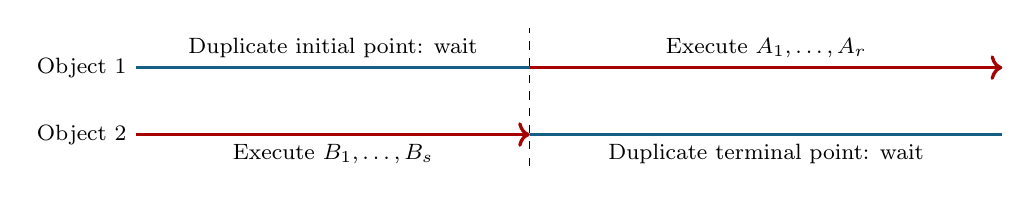
\begin{tikzpicture}[x=1cm,y=1cm]
\node[left] at (0,.65){\footnotesize Object 1};
\node[left] at (0,-.2){\footnotesize Object 2};
\draw[thick,accent] (0,.65)--(5,.65);
\node[above] at (2.5,.65){\footnotesize Duplicate initial point: wait};
\draw[->,very thick,red!65!black] (5,.65)--(11,.65);
\node[above] at (8,.65){\footnotesize Execute $A_1,\ldots,A_r$};
\draw[->,very thick,red!65!black] (0,-.2)--(5,-.2);
\node[below] at (2.5,-.2){\footnotesize Execute $B_1,\ldots,B_s$};
\draw[thick,accent] (5,-.2)--(11,-.2);
\node[below] at (8,-.2){\footnotesize Duplicate terminal point: wait};
\draw[dashed] (5,-.6)--(5,1.15);
\end{tikzpicture}\end{center}
\footnotesize The endpoints already occur in the original sequences. Only copies are inserted;
no original constituent is deleted or reordered. The horizontal axis denotes execution order.
\end{frame}

\begin{frame}{Theorem 2: proof and subsequent work}
\small
\textbf{Proof.} The nonempty initial subpath places $s_1$ outside the entire image of $P_2$.
Thus object 1 waiting at $s_1$ is disjoint from every constituent $B_k$ of object 2.
\par\medskip
Similarly, the nonempty terminal subpath places $e_2$ outside the entire image of $P_1$.
Object 2 waiting at $e_2$ is therefore disjoint from every constituent $A_k$ of object 1.
Consequently every pair in Eq. (29) is interference-free.
\par\medskip
Concatenating each object's components only adds repetitions of point paths to the original.
Both original paths are therefore completed in their original movement order.
There are finitely many pairs; finite execution of each pair gives finite total duration.
\hfill$\square$
\par\medskip
\textbf{Scope.} This is a \textbf{sufficient condition} for existence.
It asserts neither necessity nor minimum makespan. The proof uses the entire interference set,
so multiple interference components require no separate local priority assignments.
\par\medskip
\textbf{Subsequent work.} Wait duplication first establishes a safe paired path.
Using sweep merging to reduce stops and waiting is left for later.
\par\smallskip\footnotesize
For bodies of nonzero size, replace the path-intersection test in Eq. (27) with occupancy and
sweep-interference tests, retaining the same proof structure.
\end{frame}

\begin{frame}{$n$ moving objects: interference with all other paths}
\small
Let $n$ be finite. Each $P_i:[0,1]\to Q$ is a continuous simple path represented by finitely many
point paths and moving subpaths. Extend the two-object definition as follows.
\begin{equation}
 C_i=\left\{u\in[0,1]:P_i(u)\in
 \bigcup_{j\ne i}\operatorname{im}P_j\right\},
 \qquad i=1,\ldots,n.
 \tag{30}
\end{equation}
Thus $C_i$ includes \textbf{every part interfering with any other object's full path}.
For nonempty $C_i$, set $a_i=\min C_i$, $b_i=\max C_i$ and define
\begin{equation}
 P_i^-=P_i|_{[0,a_i)},\qquad P_i^+=P_i|_{(b_i,1]}.
 \tag{31}
\end{equation}
\textbf{Theorem 3 assumption.} Every path has nonempty initial and terminal subpaths.
Consequently $s_i=P_i(0)$ and $e_i=P_i(1)$ satisfy
\begin{equation}
 \{s_i,e_i\}\cap\bigcup_{j\ne i}\operatorname{im}P_j=\varnothing
 \qquad(i=1,\ldots,n).
 \tag{32}
\end{equation}
\footnotesize An object with $C_i=\varnothing$ has a full path disjoint from all others and can be
included in the construction. Use the first and last boundaries even for disconnected interference sets.
Starts and goals must be safe against all other paths, not selected independently for separate pairs.
\end{frame}

\begin{frame}{Theorem 3: interference-free tuples by wait duplication}
\small
\textbf{Claim.} Under these conditions, point-path duplication alone constructs
an \textbf{interference-free sequence of $n$-component path tuples} completing all original paths.
Two-object paired paths are the special case $n=2$.
\par\medskip
Write object $i$'s constituent sequence as $A_{i,1},\ldots,A_{i,r_i}$.
Send objects in order $1,2,\ldots,n$. During constituent $k$ of object $i$, use the tuple
\begin{equation}
 T_{i,k}=\bigl(
 \langle e_1\rangle,\ldots,\langle e_{i-1}\rangle,
 A_{i,k},
 \langle s_{i+1}\rangle,\ldots,\langle s_n\rangle
 \bigr)
 \tag{33}
\end{equation}
Earlier objects duplicate their terminal point paths; later objects duplicate their initial point paths.
\begin{center}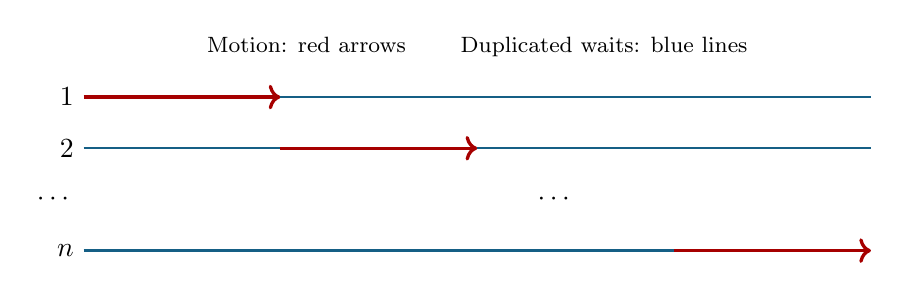
\begin{tikzpicture}[x=1cm,y=.65cm]
\foreach \y/\lab in {3/1,2/2,1/{\cdots},0/n}
 {\node[left] at (0,\y){$\lab$};}
\draw[->,very thick,red!65!black] (0,3)--(2.5,3);
\draw[thick,accent] (2.5,3)--(10,3);
\draw[thick,accent] (0,2)--(2.5,2);
\draw[->,very thick,red!65!black] (2.5,2)--(5,2);
\draw[thick,accent] (5,2)--(10,2);
\node at (6,1){$\cdots$};
\draw[thick,accent] (0,0)--(7.5,0);
\draw[->,very thick,red!65!black] (7.5,0)--(10,0);
\node[above] at (5,3.6){\footnotesize Motion: red arrows \qquad Duplicated waits: blue lines};
\end{tikzpicture}\end{center}
\footnotesize The horizontal axis denotes tuple order, not time. Each original constituent is used once,
in its original order; all added constituents are copies of an initial or terminal point path.
\end{frame}

\begin{frame}{Theorem 3: tuple safety and completion}
\small
\textbf{Tuple safety.} Only object $i$ can move in $T_{i,k}$.
Every other object $j$ waits at $w_j=s_j$ or $w_j=e_j$.
By Eq. (32), $w_j\notin\operatorname{im}P_i$, hence
\begin{equation}
 \{w_j\}\cap\operatorname{im}A_{i,k}=\varnothing.
 \tag{34}
\end{equation}
Waiting objects are also mutually disjoint. For $j\ne\ell$,
$w_\ell\in\operatorname{im}P_\ell$ while $w_j\notin\operatorname{im}P_\ell$, so
$w_j\ne w_\ell$. All component pairs in each tuple are therefore interference-free.
\par\medskip
\textbf{Induction on completed objects.} Initially, all objects occupy their starts.
Suppose the first $i-1$ objects have completed and wait at their goals.
Executing $T_{i,1},\ldots,T_{i,r_i}$ from Eq. (33) safely completes object $i$'s path,
by tuple safety. All later objects still wait at their starts.
The same state structure therefore holds with $i$ completed objects.
Induction over finite $n$ proves completion of all objects.
\par\medskip
Each object's concatenated components only add point-path repetitions to its original sequence.
There are $\sum_i r_i$ tuples, a finite number. If each tuple executes in finite time, the total duration
is finite.\hfill$\square$
\par\medskip\footnotesize
The theorem establishes \textbf{existence under the stated sufficient condition}, not feasibility for arbitrary paths
or efficiency. For bodies of nonzero size, use occupancy and sweeps in the same conditions.
Efficiency improvements through sweep merging remain subsequent work.
\end{frame}

\end{document}
